\chapter{System Architecture and Implementation}
\label{chap:architecture}

\section{Architectural Overview}

\subsection{Eight-Layer Pipeline and Graceful Degradation}

\textbf{CITRA} organizes manuscript verification into an acyclic sequence of eight software layers, summarized in Table~\ref{tab:layers} and illustrated in Figure~\ref{fig:architecture}. Each layer accepts typed data structures and emits explicit status metadata so individual stages can be unit-tested or replaced independently.

{\setlength{\tabcolsep}{3.5pt}
\begin{longtable}{|L{0.18}|L{0.34}|L{0.48}|}
\caption{Responsibilities and core Python/TypeScript modules of the eight system layers.}\label{tab:layers}\\
\hline
\textbf{Layer} & \textbf{Principal Modules} & \textbf{Core Responsibility} \\
\hline
\endfirsthead
\multicolumn{3}{c}{\itshape Table \thetable\ (continued from previous page)}\\
\hline
\textbf{Layer} & \textbf{Principal Modules} & \textbf{Core Responsibility} \\
\hline
\endhead
\hline
\multicolumn{3}{r}{\itshape Continued on next page}\\
\endfoot
\hline
\endlastfoot
\textbf{1. Extraction} & \texttt{document\_parser}, \texttt{grobid\_parser}, \texttt{grobid\_adapter}, \texttt{docx\_parser}, \texttt{patterns/*}, \texttt{style\_detector} & Parse PDF, DOCX, BibTeX, and RIS inputs into body text, contextual in-text markers, and bibliography entries across \textbf{12 styles}. \\
\hline
\textbf{2. Merging} & \texttt{integrity\_pipeline.\_merge\_citations} & Deduplicate in-text, bibliography, and appendix citations into unique referenced works while keeping all inline occurrences. \\
\hline
\textbf{3. Linking} & \texttt{citation\_linker}, \texttt{duplicate\_detector}, \texttt{statuses} & Reconstruct the bipartite graph between inline markers and bibliography entries across \textbf{7 resolution methods} and \textbf{8 statuses}. \\
\hline
\textbf{4. Retrieval} & \texttt{retrieval\_orchestrator}, \texttt{local\_db}, \texttt{link\_validator}, \texttt{html\_meta\_verifier}, 15+ clients & Route queries across offline SQLite FTS5, \textbf{15+ live APIs}, Retraction Watch, and SSRF-safe HTTP/Wayback/HTML checks. \\
\hline
\textbf{5. Matching} & \texttt{features}, \texttt{fuzzy}, \texttt{semantic}, \texttt{author\_matcher}, \texttt{venue\_normalizer} & Compute lexical similarity, metadata distances, SBERT sentence-pooled alignment, stance, and ONNX INT8 \texttt{VI}$\leftrightarrow$\texttt{EN} scores. \\
\hline
\textbf{6. Verification} & \texttt{neuro\_symbolic\_checker}, \texttt{rules}, \texttt{vn\_legal\_verifier}, \texttt{calibration} & Evaluate Order 0 + 16 symbolic rule groups (\textbf{68 rule IDs}) blended with 16D Logistic Regression and Platt calibration. \\
\hline
\textbf{7. Scoring \& Export} & \texttt{cis}, \texttt{explanation}, \texttt{bibliography\_formatter}, \texttt{docx\_exporter} & Compute the \textbf{five-component CIS}, render bilingual explanations, and export sanitized reports and repaired \texttt{.docx} files. \\
\hline
\textbf{8. Presentation} & FastAPI \texttt{api/*}, React/TypeScript \texttt{web/src/*} & Serve SSE progress, six diagnostic report views, classroom analytics, inline teacher overrides, and admin health controls. \\
\hline
\end{longtable}
}

\begin{figure}[H]
    \centering
    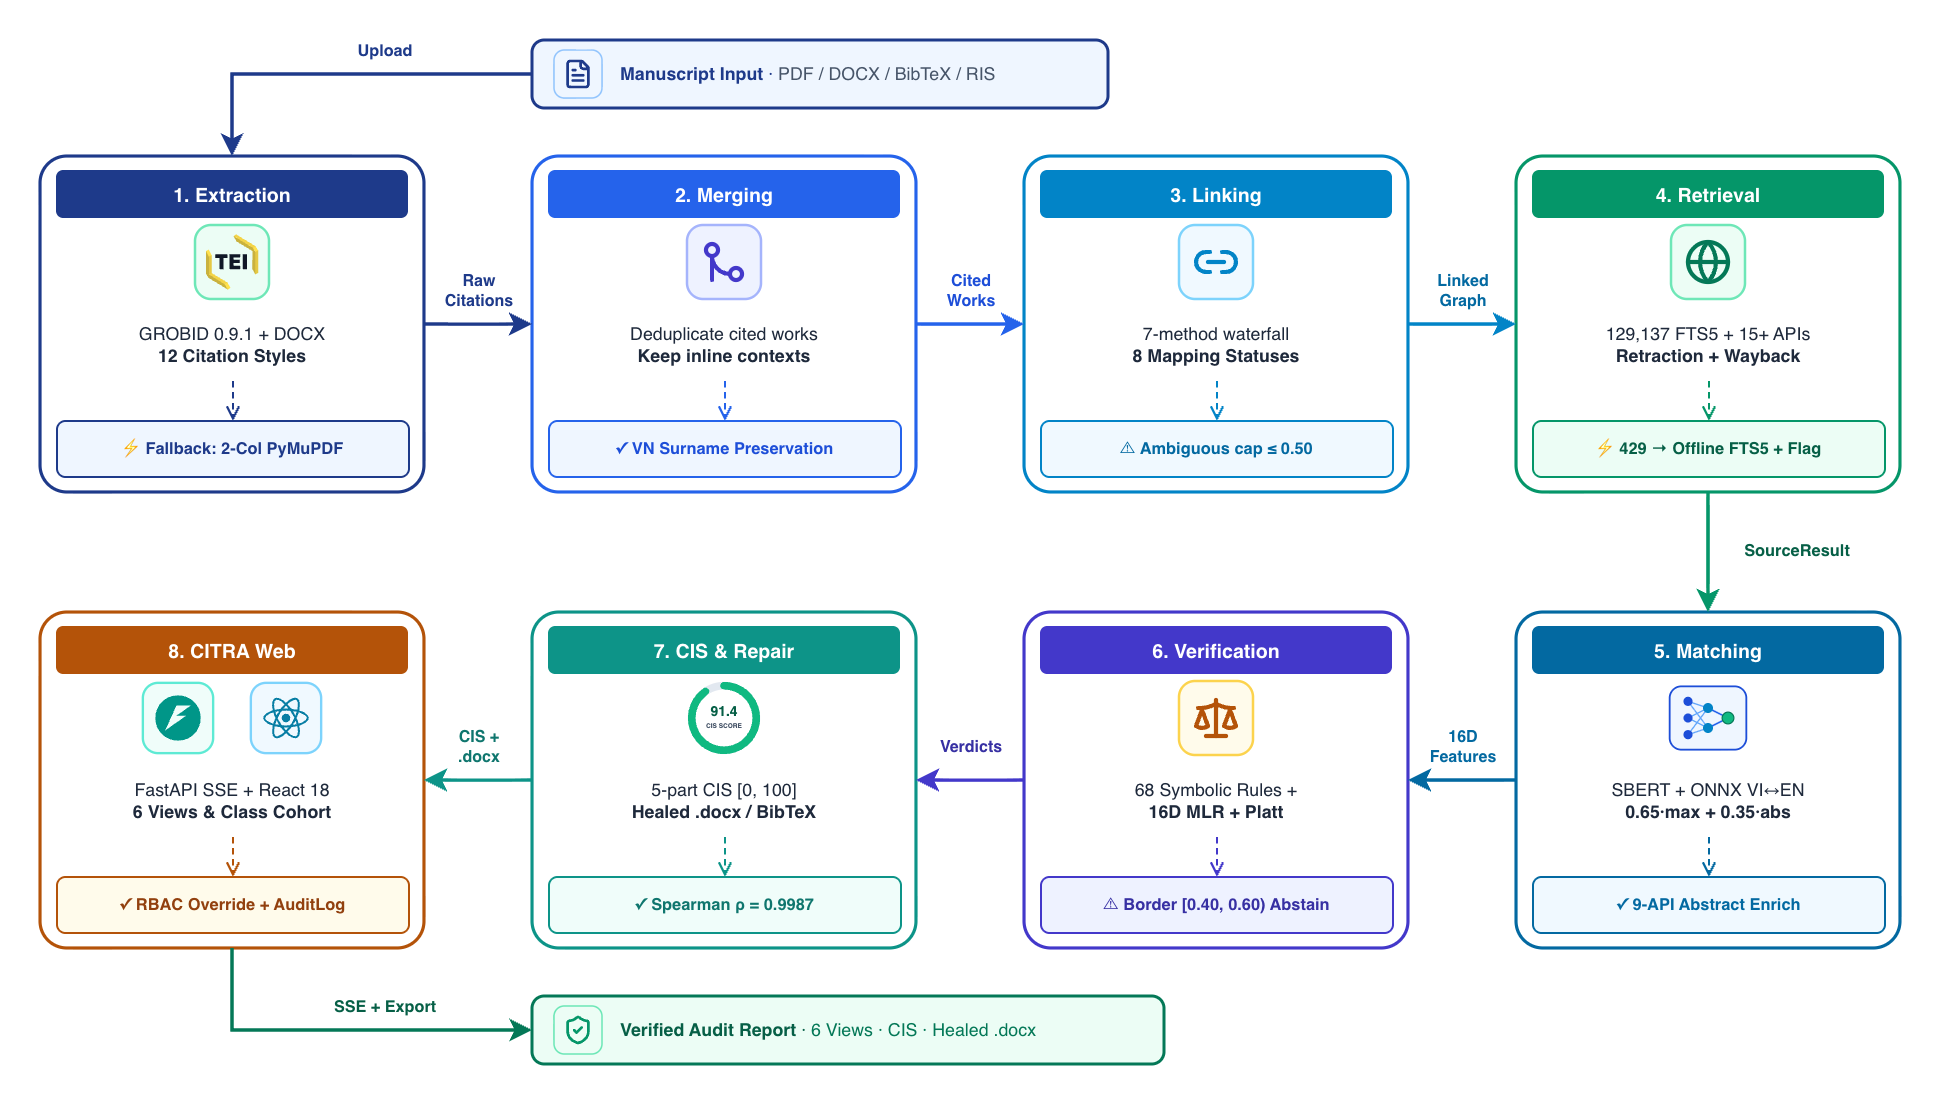
\includegraphics[width=\textwidth,keepaspectratio]{picture/figures/fig4_1_architecture.png}
    \caption[Eight-layer software architecture and graceful degradation contracts]{Eight-layer software architecture of CITRA (\texttt{v3.90.9}) showing inter-layer contracts and graceful degradation fallbacks.}
    \label{fig:architecture}
\end{figure}

Every layer enforces a strict \emph{graceful degradation contract}. If the GROBID container is unreachable, Layer 1 falls back automatically to two-column PyMuPDF and regex parsing. Similarly, if live registries return HTTP 429 or time out, Layer 4 falls back to the 129,137-record offline FTS5 index and records \texttt{api\_exhausted = True}, while Layer 6 emits \texttt{unresolved} rather than guessing whenever evidence remains incomplete.

\subsection{Software Design Patterns}

Five classical object-oriented and cloud resilience patterns keep the codebase modular and maintainable:
\begin{itemize}
    \item \textbf{Strategy and Priority Registry (\texttt{extraction/patterns/}):} Twelve citation-style parsers inherit from the \texttt{CitationFormat} base class and register integer priorities so style-specific rules remain isolated from the document reader.
    \item \textbf{Adapter (\texttt{grobid\_adapter.py} \& API Clients):} Heterogeneous external formats (GROBID TEI-XML, Crossref JATS XML, OpenAlex inverted abstract indices, arXiv Atom XML, and BibTeX) are normalized into uniform internal \texttt{Citation} and \texttt{ScholarlyCandidate} objects.
    \item \textbf{Chain of Responsibility (\texttt{CitationLinker} \& \texttt{SymbolicRules}):} Both the seven-method linker and the 16-group symbolic verifier evaluate ordered handlers and short-circuit as soon as a decisive condition fires.
    \item \textbf{Circuit Breaker and Token-Bucket Rate Limiter (\texttt{retrieval/}):} Each external API client is wrapped in a state machine (\texttt{closed} $\rightarrow$ \texttt{open} $\rightarrow$ \texttt{half\_open}) and a thread-safe rate limiter so a slow or failing upstream provider is temporarily bypassed without stalling concurrent essays.
    \item \textbf{Singleflight Request Coalescing:} Identical normalized queries arriving concurrently across batch uploads share a single in-flight HTTP coroutine before persisting the result in \texttt{citation\_cache}.
\end{itemize}

\section{Extraction Layer}

\subsection{Multi-Format Document Parsing}

Manuscript ingestion (\texttt{DocumentParser}) handles four input formats: PDF, DOCX, BibTeX, and RIS. For PDF files, the primary \texttt{grobid\_hybrid} path submits the binary stream to GROBID \texttt{0.9.1-crf}~\cite{Lopez2009}, extracting body paragraphs, inline \texttt{<ref type="bibr">} pointers, sentence windows, and \texttt{<biblStruct>} entries. Two post-processors correct recurring student-report artifacts in GROBID output: (1) a \emph{table-of-contents (TOC) and dot-leader filter} discards numbered chapter headings that mimic numbered references, and (2) a \emph{regex field-enrichment pass} recovers URLs, publishers, Vietnamese statutory codes, and humanities page ranges omitted from TEI-XML tags.

When GROBID is disabled or encounters non-standard word-processor layouts, \texttt{DocumentParser} falls back to a two-column geometry-aware PyMuPDF~\cite{PyMuPDF2024} and \texttt{pdfplumber}~\cite{Pdfplumber2024} pipeline. Pages with near-zero extractable character density trigger selective Tesseract Vietnamese/English OCR, whereas legacy Vietnamese encodings (VNI and TCVN3) are normalized to NFC Unicode. Native \texttt{.docx} manuscripts are parsed directly via \texttt{python-docx} paragraph styles and XML numbering properties without intermediate PDF conversion loss.

\subsection{Twelve Citation Style Modules and Style Detection}

Bibliography entries and inline markers are matched against twelve modular conventions listed in priority order in Table~\ref{tab:styles} and depicted in Figure~\ref{fig:extraction}. Integer priorities resolve syntactic overlaps (such as bracketed ordinals shared by IEEE, ACM, and Vancouver). In parallel, \texttt{StyleDetector} scores document-wide structural ratios to output a \texttt{StyleProfile} (\texttt{APA-like}, \texttt{IEEE-like}, \texttt{MIXED}, or \texttt{UNKNOWN}); documents mixing incompatible conventions above $30\%$ receive a style-inconsistency flag.

{\setlength{\tabcolsep}{3.5pt}
\begin{longtable}{|L{0.16}|C{0.12}|L{0.33}|L{0.39}|}
\caption{Twelve registered citation style extractors and their structural patterns.}\label{tab:styles}\\
\hline
\textbf{Style} & \textbf{Priority} & \textbf{In-Text Marker Pattern} & \textbf{Bibliography Entry Pattern} \\
\hline
\endfirsthead
\multicolumn{4}{c}{\itshape Table \thetable\ (continued from previous page)}\\
\hline
\textbf{Style} & \textbf{Priority} & \textbf{In-Text Marker Pattern} & \textbf{Bibliography Entry Pattern} \\
\hline
\endhead
\hline
\multicolumn{4}{r}{\itshape Continued on next page}\\
\endfoot
\hline
\endlastfoot
\textbf{APA (7th)} & \textbf{100} & \textit{(Author et al., 2020)}, \textit{Author (2020a)} & Author, A. B. (2020). Title of work. \textit{Venue, 12}(3), 45--67. \\
\hline
\textbf{IEEE} & \textbf{90} & \textit{[1]}, \textit{[1, 2]}, \textit{[1]--[3]} & [1] A. Author, ``Title,'' \textit{Venue}, vol.\ 1, pp.\ 1--10, 2020. \\
\hline
\textbf{ACM} & 88 & \textit{[1]}, \textit{[Author 2020]} & [1] Author Name. 2020. Title. In \textit{Proc.\ ACM}, 1--10. \\
\hline
\textbf{Harvard} & 85 & \textit{(Author, 2020)}, \textit{(Author 2020: 15)} & Author, A. (2020) \textit{Title}. Place: Publisher. \\
\hline
\textbf{Vancouver} & 80 & \textit{[1]}, \textit{(1--3)} & 1. Author AB. Title. \textit{Venue}. 2020;12(1):10--20. \\
\hline
\textbf{Nature} & 78 & Superscript / \textit{[1]} & 1. Author, A. Title. \textit{Nature} \textbf{580}, 100--105 (2020). \\
\hline
\textbf{CSE} & 77 & \textit{(Author 2020)}, superscript & Author AB. 2020. Title. \textit{Venue}. 12(1):10--20. \\
\hline
\textbf{ACS} & 76 & \textit{(1)}, superscript & (1) Author, A. B. Title. \textit{J.\ Am.\ Chem.\ Soc.} \textbf{2020}, \textit{142}, 1--5. \\
\hline
\textbf{AMA} & 75 & Superscript / \textit{[1]} & 1. Author AB. Title. \textit{JAMA}. 2020;323(1):1--10. \\
\hline
\textbf{Chicago} & 70 & \textit{(Author 2020, 45)}, footnote & Author, First. 2020. \textit{Title}. Place: Publisher. \\
\hline
\textbf{MLA (9th)} & 70 & \textit{(Author 45)}, \textit{(Author and Coauthor 12)} & Author, First. ``Title.'' \textit{Venue}, vol.\ 1, no.\ 2, 2020, pp.\ 1--15. \\
\hline
\textbf{VN Legal} & \textbf{Rule} & \begin{vietnamese}\textit{(Luật số 20/2023/QH15)}\end{vietnamese} & \begin{vietnamese}Quốc hội / Chính phủ. (2023). \textit{Luật / Nghị định / Thông tư}.\end{vietnamese} \\
\hline
\end{longtable}
}

\begin{figure}[H]
    \centering
    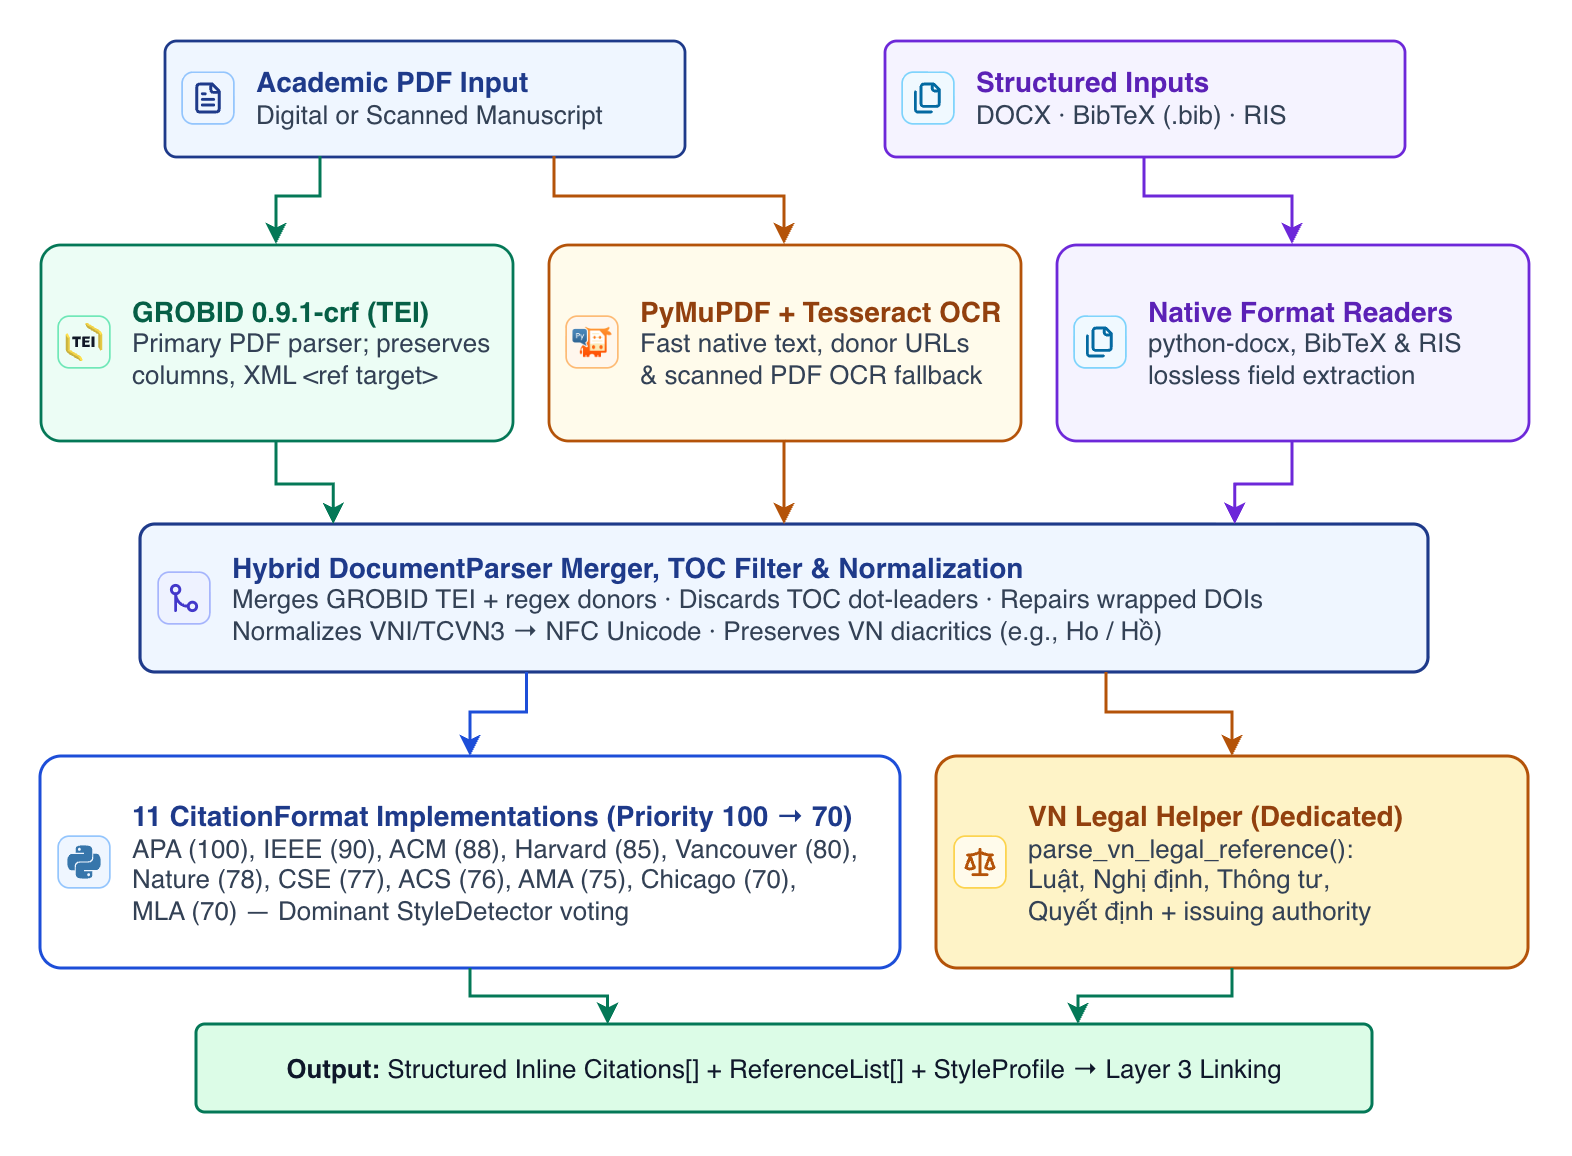
\includegraphics[width=\textwidth,keepaspectratio]{picture/figures/fig4_2_extraction.png}
    \caption[Multi-format extraction pipeline across PDF, DOCX, BibTeX, and RIS]{Extraction layer architecture combining GROBID \texttt{0.9.1-crf} TEI-XML, TOC filtering, two-column PyMuPDF fallback, selective OCR, and twelve style parsers.}
    \label{fig:extraction}
\end{figure}

\section{Merging and Bidirectional Linking}

\subsection{Work-Level Citation Merging}

Extraction yields three raw lists: body in-text markers, bibliography entries, and appendix citations. \texttt{IntegrityPipeline.\_merge\_citations} fuses matching markers and bibliography entries into a deduplicated set of unique referenced works while keeping every inline occurrence attached as a contextual observation. Short Vietnamese family names (such as \textit{Le}, \textit{Vo}, \textit{Do}, \textit{Ho}, and \textit{Ly}) are explicitly preserved during surname normalization so two-letter Vietnamese surnames are never stripped as initials. Compound markers such as \texttt{[9, 10]} or \texttt{(Vaswani et al., 2017; Devlin et al., 2019)} are expanded into individual edges, and composite numbered entries (\texttt{[14] a) ... b) ...}) are split into sub-indexed items (\texttt{14a}, \texttt{14b}).

\subsection{Seven-Method Linker and Eight Mapping Statuses}

Internal structural integrity requires a coherent bipartite graph between inline claims and the reference list. As shown in Figure~\ref{fig:linking}, \texttt{CitationLinker} runs a seven-stage resolution waterfall (plus instructor override) ordered by reliability in Table~\ref{tab:mapping-methods}, and assigns one of eight \texttt{MappingStatus} labels in Table~\ref{tab:mapping-statuses}. Duplicate bibliography entries are detected via exact DOI/arXiv match or $\ge 0.92$ combined title--author--year similarity. When \texttt{ambiguous\_mapping} occurs (for example, two papers by the same first author in the same year lacking \texttt{2024a}/\texttt{2024b} suffixes), downstream verification caps confidence at $0.50$ and forces \texttt{unresolved}.

\begin{figure}[H]
    \centering
    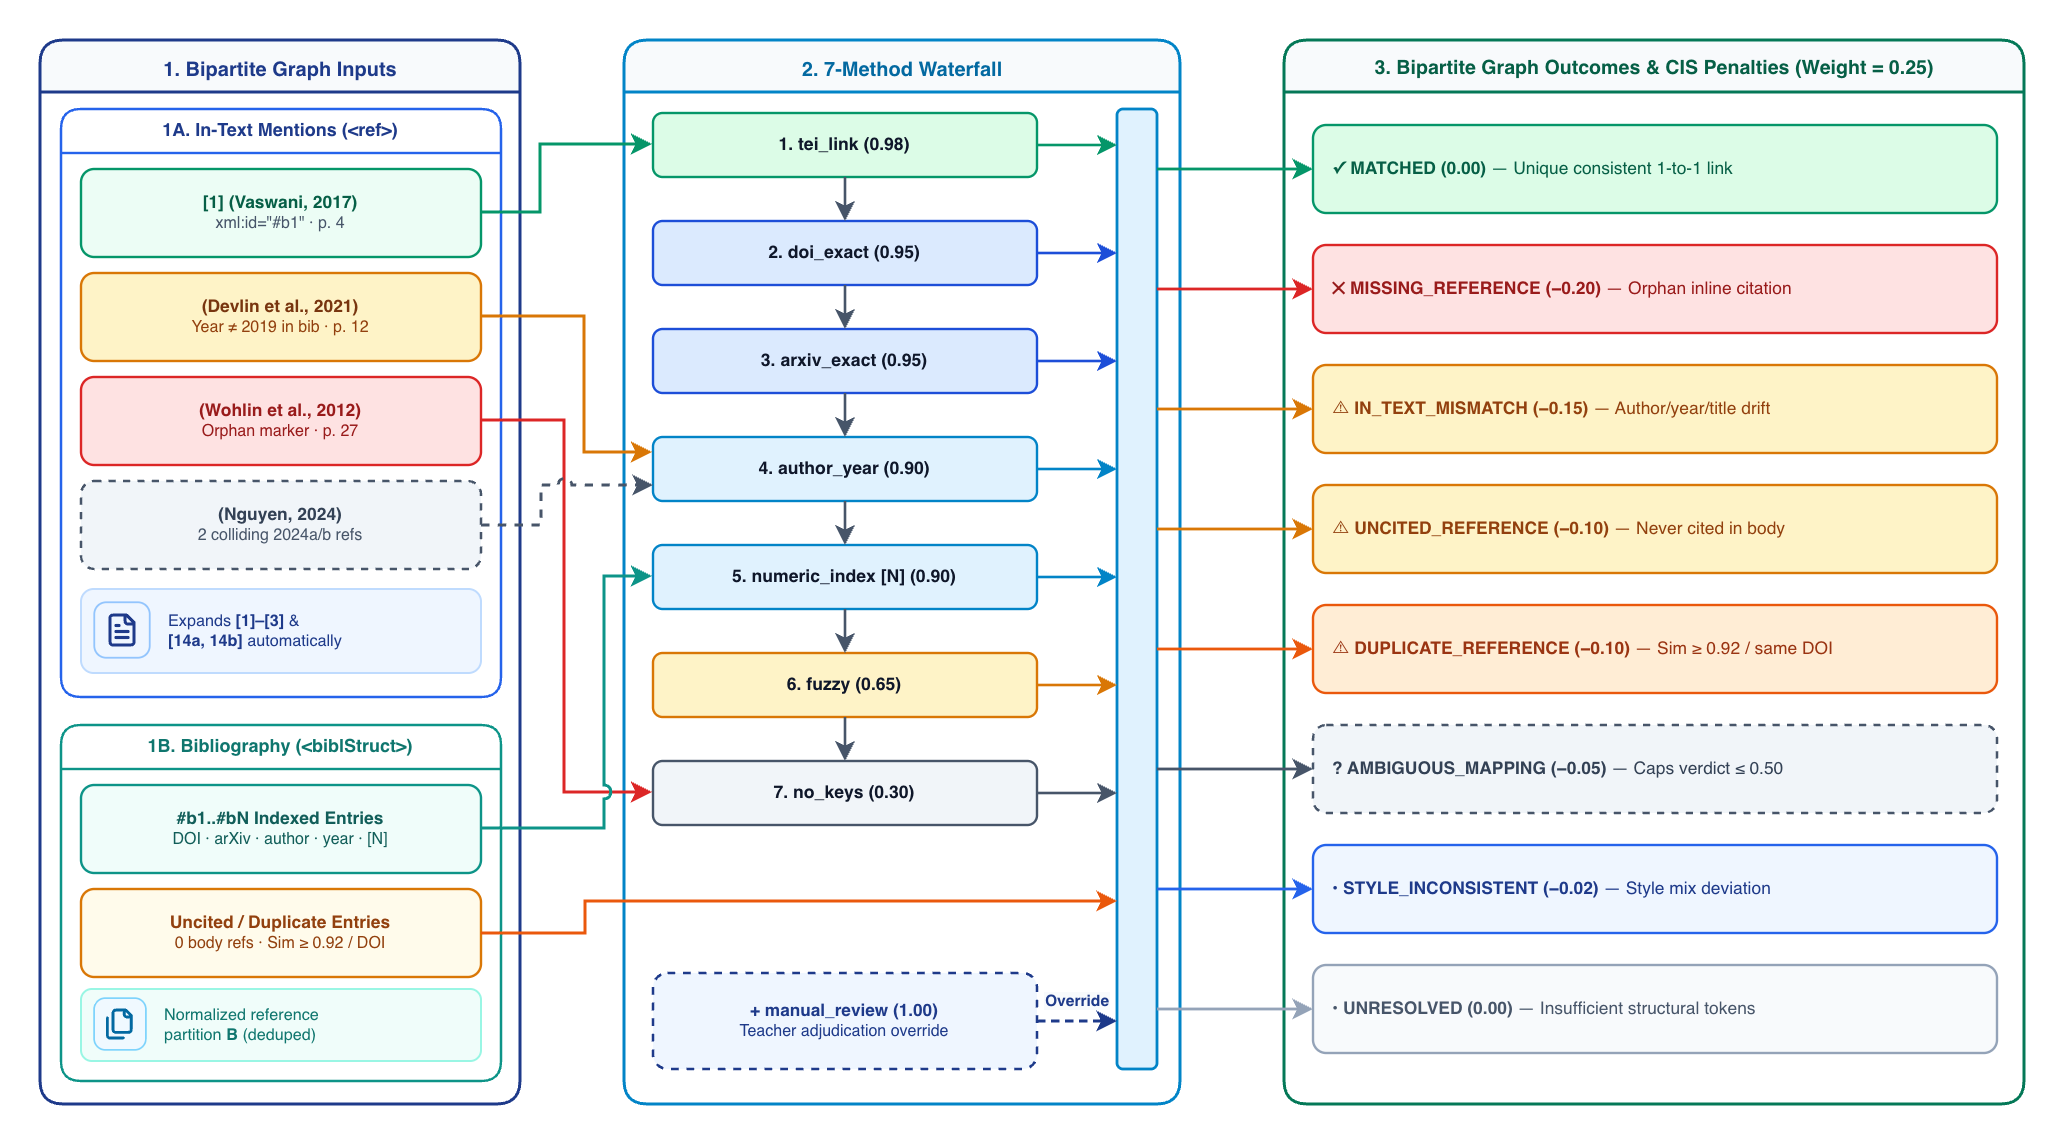
\includegraphics[width=\textwidth,keepaspectratio]{picture/figures/fig4_3_linking.png}
    \caption[Seven-method bidirectional citation linking waterfall and eight mapping statuses]{Bidirectional citation linking waterfall across seven automated resolution methods and the resulting eight structural mapping statuses.}
    \label{fig:linking}
\end{figure}

{\setlength{\tabcolsep}{3.5pt}
\begin{longtable}{|L{0.25}|C{0.15}|L{0.60}|}
\caption{Ordered resolution methods in \texttt{CitationLinker}.}\label{tab:mapping-methods}\\
\hline
\textbf{Method} & \textbf{Default Conf.} & \textbf{Matching Criterion} \\
\hline
\endfirsthead
\multicolumn{3}{c}{\itshape Table \thetable\ (continued from previous page)}\\
\hline
\textbf{Method} & \textbf{Default Conf.} & \textbf{Matching Criterion} \\
\hline
\endhead
\hline
\multicolumn{3}{r}{\itshape Continued on next page}\\
\endfoot
\hline
\endlastfoot
\textbf{\texttt{tei\_link}} & \textbf{0.98} & Direct GROBID TEI-XML \texttt{xml:id} pointer from inline \texttt{<ref>} to \texttt{<biblStruct>}. \\
\hline
\textbf{\texttt{doi\_exact}} & \textbf{0.95} & Identical normalized DOI present in both inline marker and reference entry. \\
\hline
\textbf{\texttt{arxiv\_exact}} & \textbf{0.95} & Identical canonical \texttt{arXiv} identifier present on both sides. \\
\hline
\textbf{\texttt{author\_year}} & 0.90 & Normalized surname(s), year, and optional suffix (\texttt{a}--\texttt{f}) agree (including MLA author--page inference). \\
\hline
\textbf{\texttt{numeric\_index}} & 0.90 & Bracketed or superscript ordinal (or expanded range \texttt{[1]--[3]}) matches bibliography index. \\
\hline
\textbf{\texttt{fuzzy}} & 0.65 & Partial title or author token overlap above fallback threshold when exact keys are missing. \\
\hline
\textbf{\texttt{no\_keys}} & 0.30 & Insufficient disambiguating keys or tie across multiple entries (\texttt{ambiguous\_mapping}). \\
\hline
\textbf{\texttt{manual\_review}} & \textbf{1.00} & Link explicitly adjudicated by an authorized instructor. \\
\hline
\end{longtable}
}

{\setlength{\tabcolsep}{3.5pt}
\begin{longtable}{|L{0.28}|C{0.15}|C{0.14}|L{0.43}|}
\caption{Eight structural mapping statuses and their CIS rubric penalties.}\label{tab:mapping-statuses}\\
\hline
\textbf{Mapping Status} & \textbf{Integrity Issue} & \textbf{CIS Penalty} & \textbf{Structural Meaning} \\
\hline
\endfirsthead
\multicolumn{4}{c}{\itshape Table \thetable\ (continued from previous page)}\\
\hline
\textbf{Mapping Status} & \textbf{Integrity Issue} & \textbf{CIS Penalty} & \textbf{Structural Meaning} \\
\hline
\endhead
\hline
\multicolumn{4}{r}{\itshape Continued on next page}\\
\endfoot
\hline
\endlastfoot
\textbf{\texttt{matched}} & No & 0.00 & Unique one-to-one link with consistent author/year metadata. \\
\hline
\textbf{\texttt{missing\_reference}} & \textbf{Yes} & \textbf{0.20} & Inline marker cites a source absent from the bibliography (orphan citation). \\
\hline
\textbf{\texttt{in\_text\_mismatch}} & \textbf{Yes} & \textbf{0.15} & Linked pair disagrees on publication year, surname, or title tokens. \\
\hline
\textbf{\texttt{uncited\_reference}} & \textbf{Yes} & \textbf{0.10} & Bibliography entry is never cited anywhere in the manuscript body. \\
\hline
\textbf{\texttt{duplicate\_reference}} & \textbf{Yes} & \textbf{0.10} & Two or more bibliography entries refer to the same publication. \\
\hline
\textbf{\texttt{ambiguous\_mapping}} & \textbf{Yes} & 0.05 & Inline marker collides equally with multiple bibliography entries. \\
\hline
\textbf{\texttt{style\_inconsistent}} & \textbf{Yes} & 0.02 & Entry or marker deviates from the manuscript's dominant style profile. \\
\hline
\textbf{\texttt{unresolved}} & No & 0.00 & Insufficient structural tokens to classify link state. \\
\hline
\end{longtable}
}

\section{Federated Retrieval and URL Verification}

\subsection{Domain-Aware Multi-Tier Orchestration}

Rather than broadcasting every reference to every external API, \texttt{Retrieval\allowbreak Orchestrator} routes queries through the tiered architecture shown in Figure~\ref{fig:retrieval}:
\begin{enumerate}
    \item \textbf{Pre-Screening:} Pure web URLs, software repositories, IETF RFCs, PyPI packages, Hugging Face cards, and Vietnamese legal documents (\texttt{parse\_vn\_legal\_reference} + \texttt{VNLegalVerifier}) are routed directly to specialized technical/legal verifiers.
    \item \textbf{Tier 0 (Offline Sub-100\,ms Lookup):} Queries first check the 101-paper seminal whitelist (\texttt{\_KNOWN\_PAPERS}) and the local SQLite FTS5 database (\texttt{local\_papers.db}, 129,137 records covering 128,115 unique papers and 82,887 full abstracts) using Okapi BM25 across exact-title, year-constrained, and author-constrained queries.
    \item \textbf{Tier 1 (Domain-Routed Public APIs):} Using identifier cues (DOI, arXiv ID, ISBN, PMID) and lexical domain regexes (CS/AI, Biomedicine, Books, Repositories), async queries dispatch under configured token-bucket rate limits (\texttt{configs/config.yaml}). Specifically, \textbf{Crossref} ($25\text{\,req/s}$ polite pool + Retraction Watch flags), \textbf{OpenAlex} ($8\text{\,req/s}$), \textbf{DataCite}, \textbf{Global DOI RA}, \textbf{DOAJ}, and \textbf{OpenAIRE/HAL} cover general and open-access venues, while \textbf{DBLP} ($1.5\text{\,req/s}$), \textbf{arXiv} ($1.0\text{\,req/s}$), \textbf{Europe PMC} ($5.0\text{\,req/s}$), \textbf{NCBI/bioRxiv}, \textbf{OpenLibrary / Google Books} ($3.0\text{\,req/s}$), and \textbf{Wikidata / OpenCitations} cover domain-specific records.
    \item \textbf{Tier 2 (Fallback \& Abstract Recovery):} Zero-hit queries optionally consult the \textbf{Serper / SerpAPI} router, and any winning candidate lacking an abstract triggers a 9-source \texttt{\_enrich\_missing\_abstract} pass so semantic claim alignment retains abstract coverage.
\end{enumerate}

\begin{figure}[H]
    \centering
    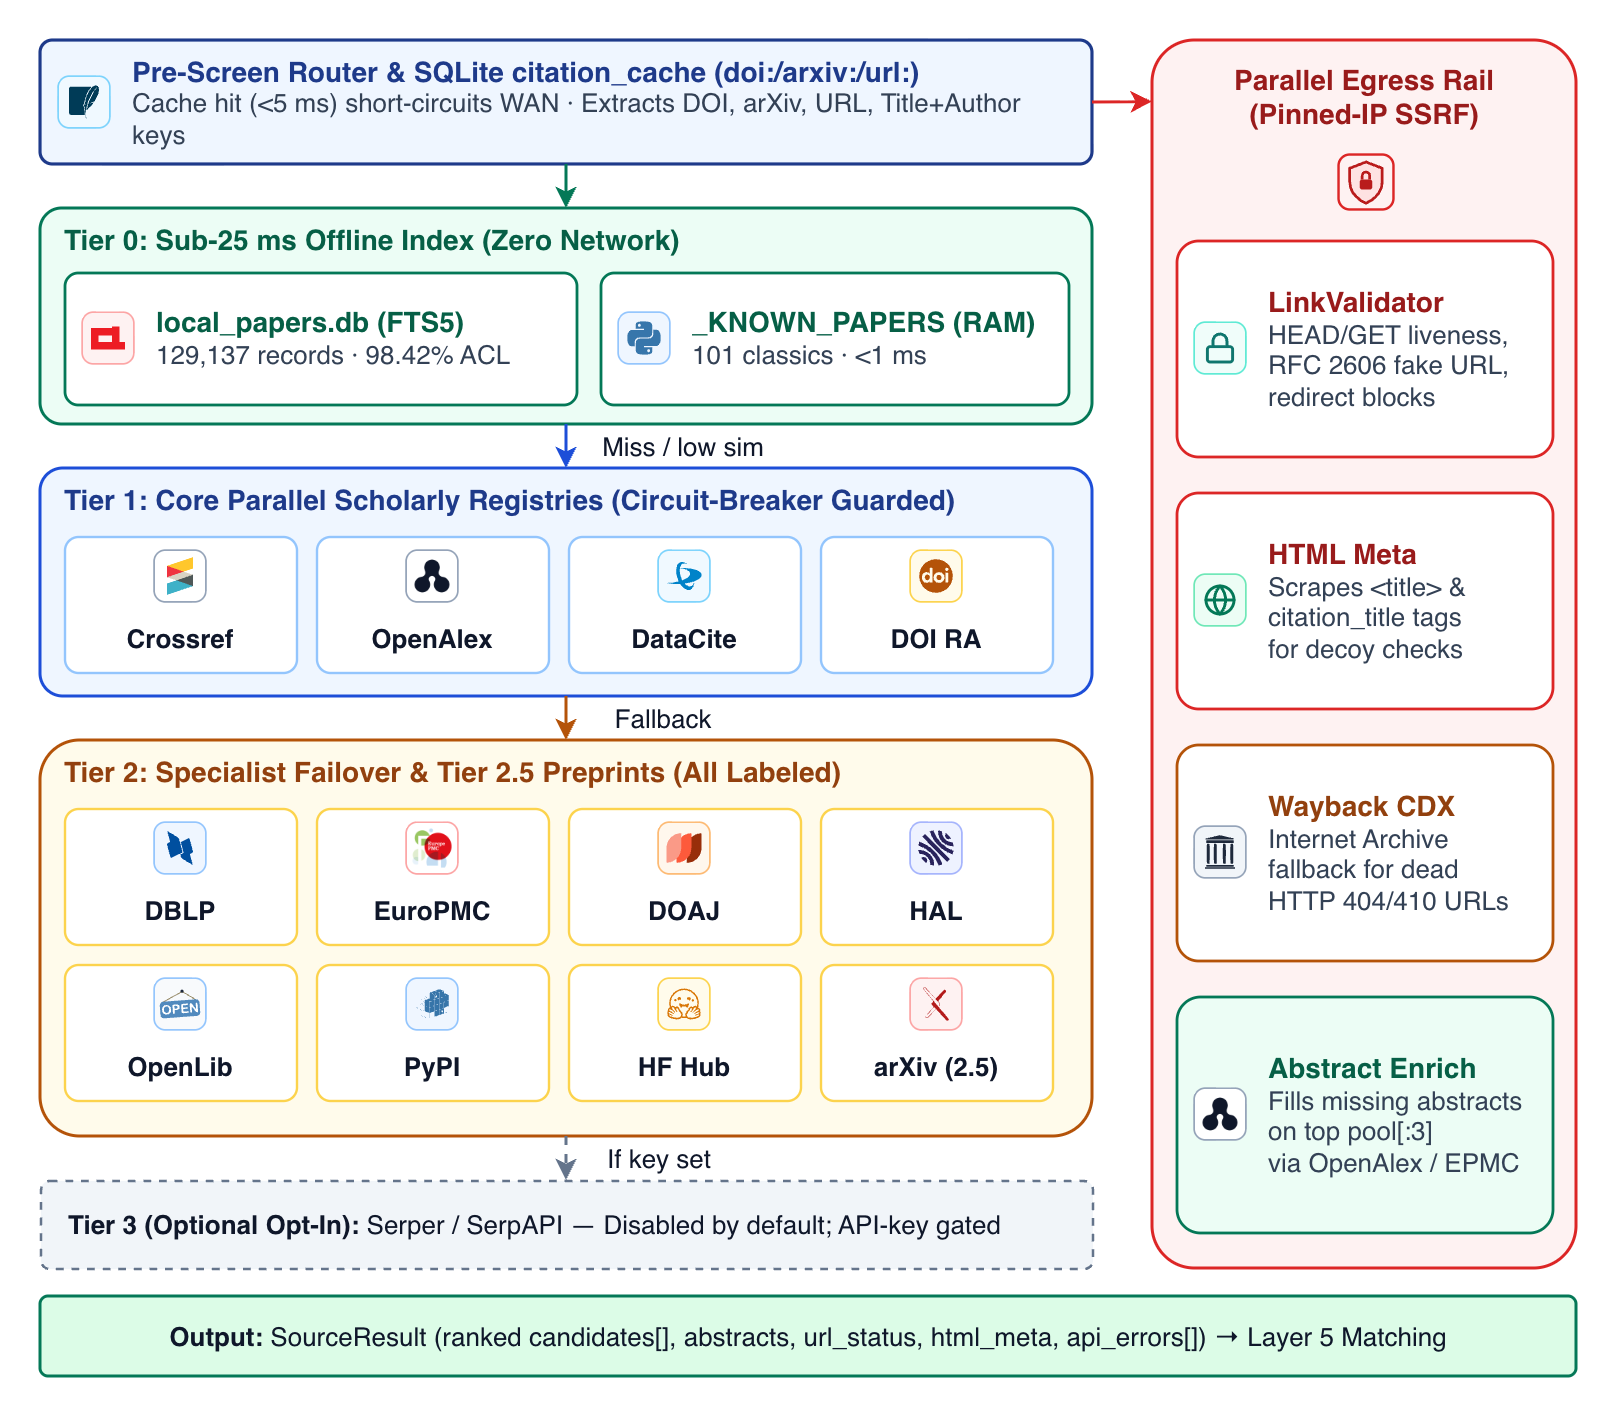
\includegraphics[width=\textwidth,keepaspectratio]{picture/figures/fig4_4_retrieval.png}
    \caption[Domain-aware multi-tier retrieval and SSRF-safe URL validation]{Domain-aware retrieval orchestration across Tier 0 (SQLite FTS5 + 101 known papers), Tier 1 (15+ live APIs), Tier 2 fallback, and parallel HTTP/Wayback/HTML verification.}
    \label{fig:retrieval}
\end{figure}

\subsection{Consensus, LinkValidator, and SafeHtmlMetaVerifier}
\label{sec:consensus}

Returned candidates are deduplicated and scored for multi-source consensus (\texttt{title\_sim} $\ge 0.90$, \texttt{author\_jaccard} $\ge 0.50$, $|\Delta y| \le 1$), inheriting abstracts across agreeing registries when one record omits abstract text. Simultaneously, \texttt{LinkValidator} probes cited URLs via pinned-IP SSRF-safe \texttt{HEAD}/\texttt{GET} requests and Internet Archive Wayback CDX lookups, assigning one of \textbf{six \texttt{LinkStatus} states}: \texttt{alive} (HTTP 200--399), \texttt{restricted\_alive} (HTTP 401/403/405/429 publisher anti-bot/paywall), \texttt{archived\_alive} (dead live link recovered in Wayback Machine), \texttt{dead\_link} (HTTP 404/410 or DNS NXDOMAIN), \texttt{fake\_domain} (RFC 2606 reserved/placeholder domains), or \texttt{unchecked}. For reachable web resources, \texttt{SafeHtmlMetaVerifier} streams up to $128\text{\,KB}$ of HTML (\texttt{MAX\_HTML\_HEAD\_BYTES = 131,072}) to extract Highwire Press (\texttt{citation\_title}, \texttt{citation\_author}, \texttt{citation\_doi}), Dublin Core, OpenGraph, and JSON-LD metadata while detecting bilingual English/Vietnamese ``Soft-404'' error pages disguised under HTTP 200 responses.

\section{Lexical, Neural, and Cross-Lingual Matching}

\subsection{Lexical and Bibliographic Field Matching}

Given the top candidate from retrieval, \texttt{FeatureCalculator} computes the structured \texttt{MatchFeatures} signals summarized in Table~\ref{tab:features}. Three domain normalizers prevent false metadata errors on legitimate scholarship. First, colon-delimited subtitle and edition stripping (\textit{2nd ed.}, \textit{Revised edition}) grants $0.95$ title similarity to clean main-title prefixes. Second, arXiv-to-proceedings year reconciliation computes \texttt{year\_distance} as the minimum $|\Delta y|$ across matching preprint and published versions of the same work, while \texttt{VenueNormalizer} expands conference and journal aliases (such as \texttt{NeurIPS} $\leftrightarrow$ \texttt{Advances in Neural Information Processing Systems}).

{\setlength{\tabcolsep}{3.5pt}
\begin{longtable}{|L{0.28}|C{0.12}|L{0.60}|}
\caption{Primary matching features computed by \texttt{FeatureCalculator} and \texttt{LinkValidator}.}\label{tab:features}\\
\hline
\textbf{Feature Name} & \textbf{Type} & \textbf{Computation} \\
\hline
\endfirsthead
\multicolumn{3}{c}{\itshape Table \thetable\ (continued from previous page)}\\
\hline
\textbf{Feature Name} & \textbf{Type} & \textbf{Computation} \\
\hline
\endhead
\hline
\multicolumn{3}{r}{\itshape Continued on next page}\\
\endfoot
\hline
\endlastfoot
\textbf{\texttt{title\_sim\_fuzzy}} & \texttt{float} & Max of normalized exact match, subtitle-prefix match ($0.95$), guarded substring ($0.90$), and RapidFuzz \texttt{token\_set\_ratio}. \\
\hline
\textbf{\texttt{title\_sim\_semantic}} & \texttt{float} & Cosine similarity between \texttt{all-MiniLM-L6-v2} embeddings of cited and candidate titles. \\
\hline
\textbf{\texttt{title\_sim\_max}} & \texttt{float} & Maximum of \texttt{title\_sim\_fuzzy} and \texttt{title\_sim\_semantic}. \\
\hline
\textbf{\texttt{author\_jaccard}} & \texttt{float} & Diacritic-folded surname overlap preserving short Vietnamese surnames (\textit{Le}, \textit{Vo}, \textit{Do}). \\
\hline
\textbf{\texttt{year\_distance}} & \texttt{int} & Minimum $|y_{\text{cited}} - y_{\text{cand}}|$ across matching preprint/edition records ($999$ if missing). \\
\hline
\textbf{\texttt{venue\_sim}} & \texttt{float} & Alias-expanded venue token similarity in $[0, 1]$ from \texttt{VenueNormalizer}. \\
\hline
\textbf{\texttt{doi\_exact\_match}} & \texttt{bool} & Exact normalized DOI match or canonical arXiv-to-publisher DOI equivalence. \\
\hline
\textbf{\texttt{source\_consensus}} & \texttt{int} & Count of independent registries returning a corroborating candidate record. \\
\hline
\textbf{\texttt{content\_alignment\_score}} & \texttt{float} & Sentence-pooled neural alignment between inline claim context and candidate title/abstract (Equation~\eqref{eq:abs-pooling}). \\
\hline
\textbf{\texttt{stance\_label}} & \texttt{str} & Claim support state (\texttt{supported}, \texttt{partially\_supported}, \texttt{neutral}, \texttt{contradiction\_risk}) via stem-specificity gating. \\
\hline
\textbf{\texttt{url\_status}} & \texttt{enum} & Six-state URL liveness (\texttt{alive}, \texttt{restricted\_alive}, \texttt{archived\_alive}, \texttt{dead\_link}, \texttt{fake\_domain}, \texttt{unchecked}). \\
\hline
\end{longtable}
}

\subsection{Dual-Encoder Semantic Alignment and Stance Analysis}

Figure~\ref{fig:matching} illustrates the dual-encoder neural matching pipeline in \texttt{SemanticMatcher}. Monolingual English claims and abstracts are encoded via Sentence-BERT (\texttt{all-MiniLM-L6-v2}, 384D)~\cite{reimers2019sbert} and pooled across abstract sentences via Equation~\eqref{eq:abs-pooling} ($0.65\max + 0.35\text{abs}$), aggregating up to eight inline occurrences per referenced work. Whenever Vietnamese diacritics are detected in the inline sentence while the retrieved abstract is in English (or vice versa), \texttt{SemanticMatcher} automatically invokes the quantized ONNX INT8 \texttt{paraphrase-multilingual-MiniLM-L12-v2} encoder~\cite{reimers2020multilingual} to compute cross-lingual similarity and extract bridged bilingual concept pairs. Claim stance and citation intent (\texttt{background}, \texttt{methodology}, \texttt{result\_comparison}) use verb-agnostic content-stem specificity gating rather than brittle reporting-verb lists, catching polarity-inverting or unrelated factual claims attached to real papers.

\begin{figure}[H]
    \centering
    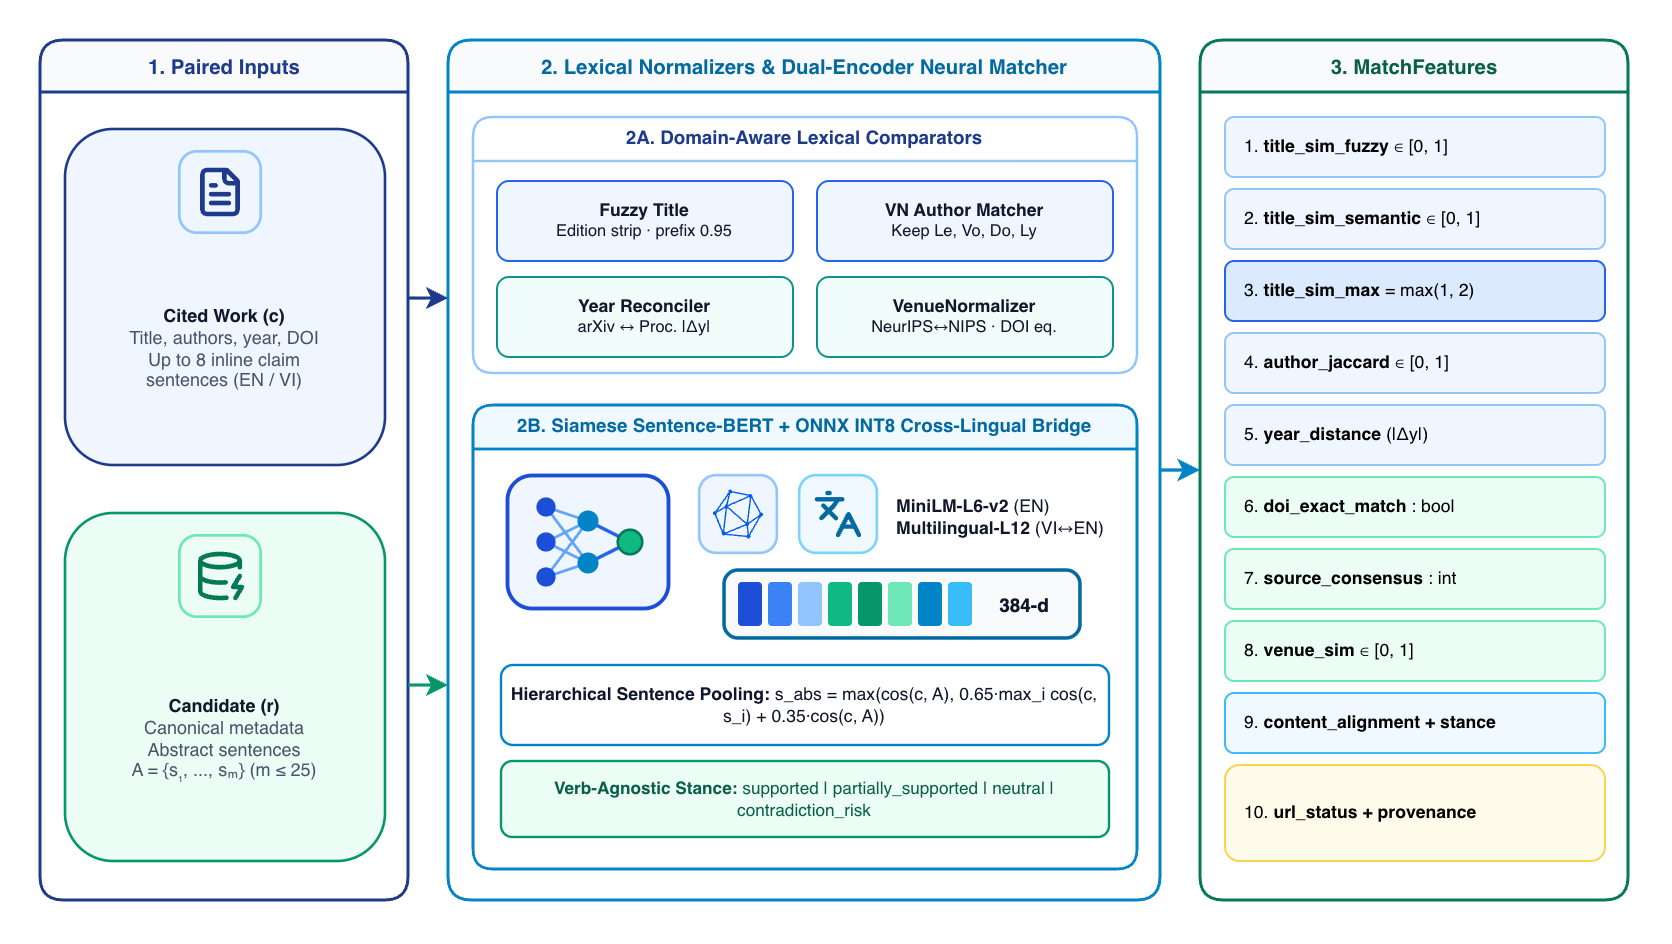
\includegraphics[width=\textwidth,keepaspectratio]{picture/figures/fig4_5_matching.png}
    \caption[Dual-encoder lexical, semantic, and cross-lingual matching architecture]{Matching layer architecture combining lexical field normalizers, Sentence-BERT sentence-pooled abstract alignment ($0.65\max + 0.35\text{abs}$), stance gating, and ONNX INT8 \texttt{VI}$\leftrightarrow$\texttt{EN} bridging.}
    \label{fig:matching}
\end{figure}

\section{Neuro-Symbolic Verification and Platt Calibration}

\subsection{Priority-Ordered Symbolic Decision Tree}

\texttt{NeuroSymbolicChecker} combines neural alignment features with a deterministic symbolic rule engine (\texttt{SymbolicRules}, containing \textbf{68 distinct \texttt{R-*} rule identifiers} across an Order 0 resource pre-screen and 16 priority-ordered scholarly rule groups) and a calibrated machine-learning scorer, as shown in Figure~\ref{fig:neurosymbolic} and detailed in Table~\ref{tab:rules}.

\begin{figure}[H]
    \centering
    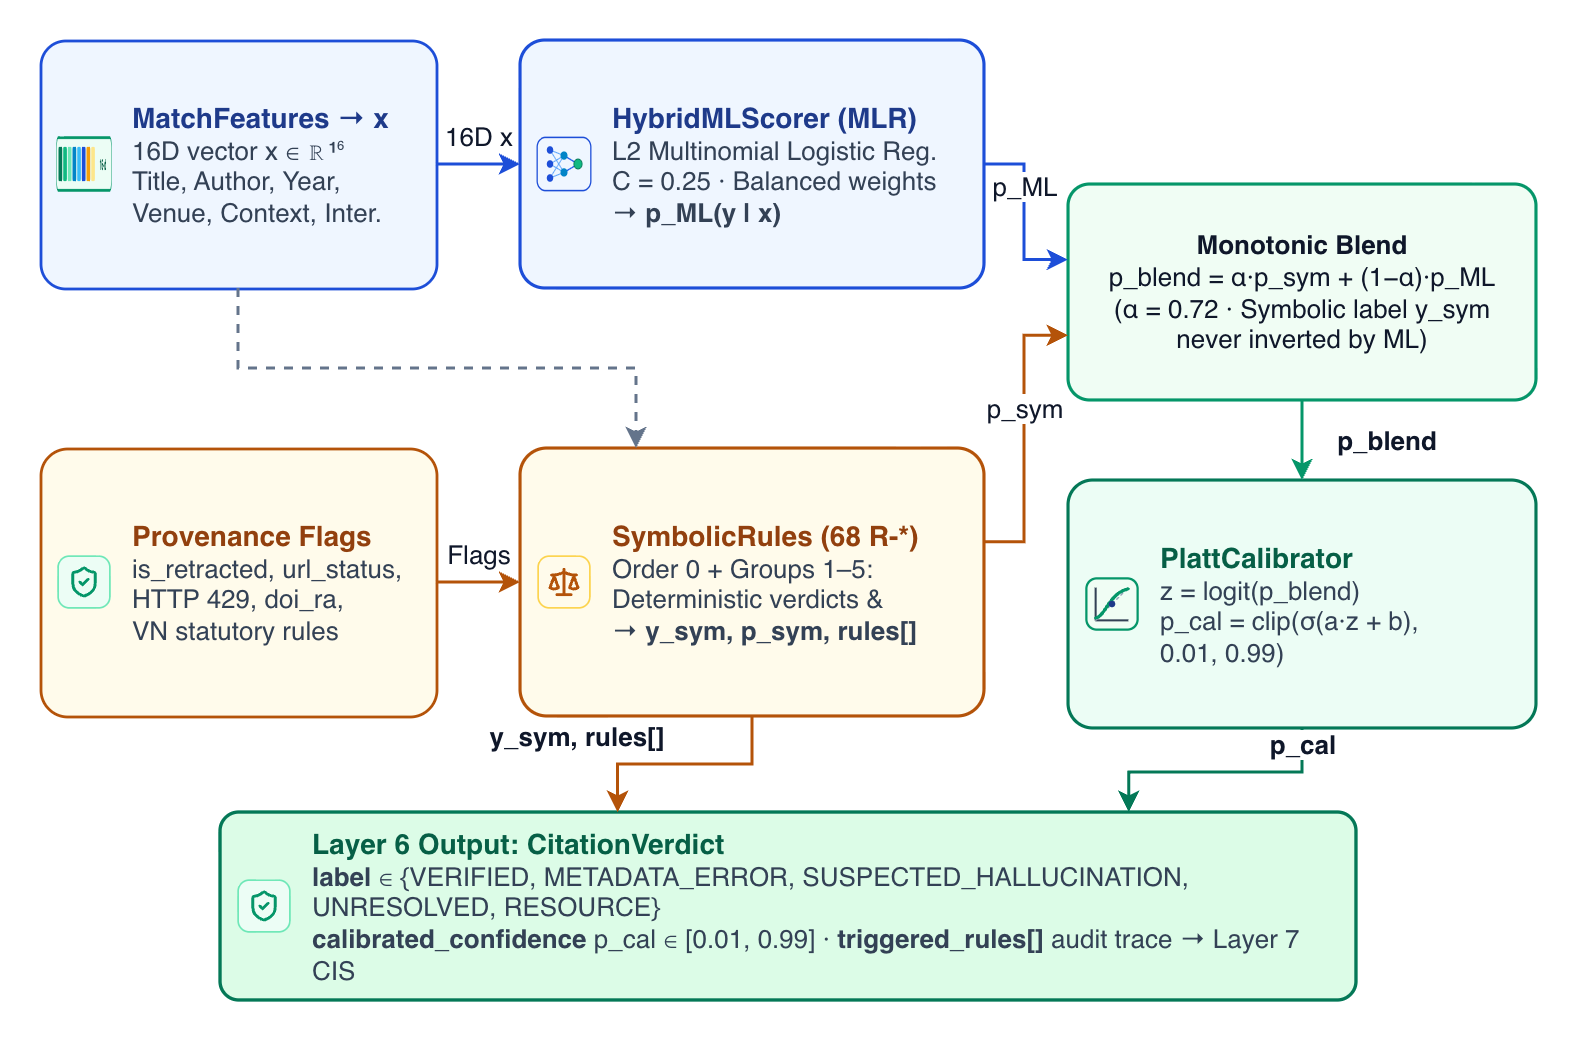
\includegraphics[width=\textwidth,keepaspectratio]{picture/figures/fig4_6_neurosymbolic.png}
    \caption[Neuro-symbolic verification engine and logit-space Platt calibration]{Neuro-symbolic verification architecture fusing the 16-group symbolic rule engine (68 rule IDs) with the 16-feature Multinomial Logistic Regression scorer and Platt calibrator.}
    \label{fig:neurosymbolic}
\end{figure}

{\setlength{\tabcolsep}{3.5pt}
\begin{longtable}{|C{0.11}|L{0.33}|L{0.56}|}
\caption{Evaluation order of symbolic pre-screening and the 16 verification rule groups (68 distinct \texttt{R-*} rule IDs).}\label{tab:rules}\\
\hline
\textbf{Group} & \textbf{Representative Rule ID(s)} & \textbf{Trigger Condition and Verdict Outcome} \\
\hline
\endfirsthead
\multicolumn{3}{c}{\itshape Table \thetable\ (continued from previous page)}\\
\hline
\textbf{Group} & \textbf{Representative Rule ID(s)} & \textbf{Trigger Condition and Verdict Outcome} \\
\hline
\endhead
\hline
\multicolumn{3}{r}{\itshape Continued on next page}\\
\endfoot
\hline
\endlastfoot
\textbf{Pre-0} & \texttt{R-URL-RESOURCE}, \texttt{R-WEB-RESOURCE}, \texttt{R-VN-LEGAL-VERIFIED}, \texttt{R-VN-LEGAL-\allowbreak MISMATCH} & Pure web documentation, software/RFC/HF artifact, or Vietnamese statute checked by \texttt{VNLegalVerifier} $\rightarrow$ \textbf{\texttt{resource}} (or \texttt{metadata\_error} if statutory authority/code conflicts). \\
\hline
\textbf{1} & \texttt{R-FAKE-URL}, \texttt{R-FABRICATED-DOI}, \texttt{R-CHIMERIC-DOI-\allowbreak MISMATCH}, \texttt{R-RETRACTED-PAPER} & RFC 2606 fake domain, unregistered DOI prefix, or real DOI resolving to an unrelated title $\rightarrow$ \textbf{\texttt{suspected\_hallucination}}; Retraction Watch flag (\texttt{is\_retracted}) $\rightarrow$ \textbf{\texttt{metadata\_error}}. \\
\hline
\textbf{2} & \texttt{R-FUTURE-YEAR}, \texttt{R-FUTURE-YEAR-\allowbreak KNOWN-AUTHOR} & Cited year exceeds current calendar year: unknown work $\rightarrow$ \textbf{\texttt{suspected\_hallucination}}; known work/author $\rightarrow$ \textbf{\texttt{metadata\_error}}. \\
\hline
\textbf{3} & \texttt{R-KNOWN-PAPER}, \texttt{R-TITLE-MISMATCH} & Matches 101-paper whitelist: full metadata \& stance agreement $\rightarrow$ \textbf{\texttt{verified}}; altered year/author/claim $\rightarrow$ \textbf{\texttt{metadata\_error}}. \\
\hline
\textbf{4} & \texttt{R-DEAD-URL}, \texttt{R-NONEXISTENT-DOI}, \texttt{R-NO-SCHOLARLY-\allowbreak RECORD} & Zero candidates while $\ge 2$ live registries returned clean HTTP 200 responses (or confirmed unarchived dead URL) $\rightarrow$ \textbf{\texttt{suspected\_hallucination}} (pure absence capped at $\le 0.88$). \\
\hline
\textbf{5} & \texttt{R-FAIL-ALL}, \texttt{R-RATE-LIMITED-\allowbreak ABSTAIN}, \texttt{R-DOI-RA-NO-CSL} & Zero candidates caused by HTTP 429 exhaustion, network outage, or valid regional DOI lacking public CSL metadata $\rightarrow$ \textbf{\texttt{unresolved}}. \\
\hline
\textbf{6} & \texttt{R-DOI-TITLE-AUTHOR} & Exact live DOI match with $\texttt{title\_sim} \ge 0.90$ and $\texttt{author\_jaccard} \ge 0.50$ $\rightarrow$ \textbf{\texttt{verified}}. \\
\hline
\textbf{7} & \texttt{R-LOCAL\_DB\_VERIFIED}, \texttt{R-LOCAL\_DB\_GOOD\_MATCH} & Offline FTS5 match ($\texttt{title\_sim\_fuzzy} \ge 0.95$, $\texttt{author\_jaccard} \ge 0.80$, $|\Delta y| = 0$) with no DOI conflict $\rightarrow$ \textbf{\texttt{verified}}. \\
\hline
\textbf{8} & \texttt{R-WELL-LINKED}, \texttt{R-WELL-LINKED-\allowbreak MODERATE} & Linked citation ($\texttt{matched}$) with strong title/author/year agreement and zero identifier contradiction $\rightarrow$ \textbf{\texttt{verified}}. \\
\hline
\textbf{9} & \texttt{R-DOI-TITLE-\allowbreak MISMATCH} & Live DOI resolves, but title similarity falls in $[0.60, 0.90)$ $\rightarrow$ \textbf{\texttt{metadata\_error}} with mismatched fields isolated. \\
\hline
\textbf{10} & \texttt{R-CONSENSUS-FULL}, \texttt{R-CONSENSUS-\allowbreak PARTIAL} & $\ge 2$ registries agree on title ($\ge 0.90$): matching author/year $\rightarrow$ \textbf{\texttt{verified}}; drifted author/year $\rightarrow$ \textbf{\texttt{metadata\_error}}. \\
\hline
\textbf{11} & \texttt{R-SINGLE-SOURCE-\allowbreak VERIFIED}, \texttt{R-BOOK-EDITION-\allowbreak VERIFIED}, \texttt{R-SINGLE-SOURCE-\allowbreak PARTIAL} & Single live registry match ($\ge 0.90$ title, $\ge 0.80$ author, $|\Delta y| \le 1$, or $\le 15\text{\,yr}$ across OpenLibrary book editions) $\rightarrow$ \textbf{\texttt{verified}}; field drift $\rightarrow$ \textbf{\texttt{metadata\_error}}. \\
\hline
\textbf{12} & \texttt{R-AMBIGUOUS-\allowbreak MAPPING} & Bipartite linker flagged \texttt{ambiguous\_mapping} $\rightarrow$ \textbf{\texttt{unresolved}} with confidence capped at $0.50$. \\
\hline
\textbf{13} & \texttt{R-CONTENT-\allowbreak ALIGNMENT}, \texttt{R-CONTENT-MISMATCH} & Strong context-to-abstract alignment rescues abbreviated titles ($\rightarrow$ \textbf{\texttt{verified}}); contradicted body claim on matched paper $\rightarrow$ \textbf{\texttt{metadata\_error}}. \\
\hline
\textbf{14} & \texttt{R-KNOWN-AUTHOR-\allowbreak TITLE-MISMATCH} & Known scholar combined with mismatched title in $[0.30, 0.90)$ $\rightarrow$ \textbf{\texttt{metadata\_error}}. \\
\hline
\textbf{15} & \texttt{R-ABSTENTION-\allowbreak BORDER}, \texttt{R-DOMAIN-EXCEPTION} & Borderline title similarity in $[0.40, 0.60)$ $\rightarrow$ \textbf{\texttt{unresolved}}; verified paper with dead external URL sets \texttt{domain\_exception = True}. \\
\hline
\textbf{16} & \texttt{R-WEAK-EVIDENCE}, \texttt{R-HALLUCINATED-\allowbreak SOURCE} & Terminal fallback ($\texttt{title\_sim} < 0.40$): $\ge 2$ clean live APIs + low author overlap $\rightarrow$ \textbf{\texttt{suspected\_hallucination}}; otherwise $\rightarrow$ \textbf{\texttt{unresolved}}. \\
\hline
\end{longtable}
}

Two provenance safeguards in \texttt{SymbolicRules} prevent overconfident false accusations. First, Group 4 (\texttt{R-NO-SCHOLARLY-RECORD}) fires only when at least two live scholarly APIs return HTTP 200 with zero matches; if APIs fail or hit HTTP 429, Group 5 forces \texttt{unresolved}. Second, when a hallucination suspicion rests purely on registry absence rather than a positive contradiction (such as a chimeric or fake DOI), post-calibration confidence is explicitly capped at $\le 0.88$ to acknowledge finite indexing coverage.

\subsection{16-Feature Logistic Regression and Platt Calibration}

To convert discrete symbolic outcomes into smooth, accurate probabilities, \texttt{HybridMLScorer} extracts a 16-dimensional feature vector $\mathbf{x} \in \mathbb{R}^{16}$ containing ten base features (\texttt{title\_sim\_fuzzy}, \texttt{title\_sim\_semantic}, \texttt{title\_sim\_max}, \texttt{author\_jaccard}, $\exp(-0.5 \min(|\Delta y|, 10))$, \texttt{doi\_exact\_match}, $\min(\text{consensus}, 4)/4$, \texttt{venue\_sim}, \texttt{content\_alignment\_signal}, \texttt{has\_candidate}) and six interaction terms (\texttt{title\_x\_author}, \texttt{title\_x\_year}, \texttt{title\_mismatch\_author}, \texttt{title\_mismatch\_year}, \texttt{doi\_mismatch\_title}, and \texttt{abstention\_zone\_indicator}).

A Multinomial Logistic Regression model ($W \in \mathbb{R}^{4 \times 16}, \mathbf{b} \in \mathbb{R}^4$, regularized at $C = 0.25$ with balanced class weights on 84,000 disjoint training citations) outputs $P_{\text{ML}}(y \mid \mathbf{x})$. In \texttt{SymbolicRules}, provenance modifiers (\texttt{R-LOCAL\_DB}: $-0.05$, \texttt{R-API\_EXHAUSTED}: $-0.10$, \texttt{R-LOCAL\_DB\_ONLY}: $-0.15$) first adjust local-only or rate-limited symbolic confidence; \texttt{HybridMLScorer} then blends symbolic confidence $C_{\text{sym}}^{(0)}$ with $P_{\text{ML}}(y_{\text{sym}} \mid \mathbf{x})$ via Equation~\eqref{eq:platt-calib} using $\alpha = 0.72$ (raised automatically to $\alpha = 0.90$ when $C_{\text{sym}}^{(0)} \ge 0.85$ and $|C_{\text{sym}}^{(0)} - P_{\text{ML}}| > 0.45$ so symbolic guardrails on retracted or fake-URL citations are never diluted). Finally, \texttt{PlattCalibrator} ($a = 1.891263, b = 1.138599$, fitted on 18,000 validation citations), document style penalties, and the $\le 0.88$ pure-absence cap produce the final calibrated confidence.

\section{Integrity Scoring and Bilingual Explanations}

\subsection{Five-Component Citation Integrity Score}

\texttt{CISCalculator.compute()} summarizes manuscript-wide citation quality as an interpretable score in $[0, 100]$. Non-scholarly \texttt{resource} entries are excluded from the academic denominator $N_{\text{acad}}$ so citing official software manuals or national laws never distorts scholarly verification ratios. For $N_{\text{acad}} \ge 1$, \texttt{metadata\_accuracy} ($s_{\text{meta}}$) applies tiered deductions across standard metadata errors ($N_{\text{meta\_std}}$, penalty $0.50$), severely incomplete references ($N_{\text{meta\_incomp}}$, penalty $0.75$), and suspected hallucinations ($N_{\text{hall}}$, penalty $1.00$), as defined in Equation~\eqref{eq:cis-meta}:
\begin{equation}\label{eq:cis-meta}
s_{\text{meta}} = \max\left(0,\; 1 - \frac{0.50\,N_{\text{meta\_std}} + 0.75\,N_{\text{meta\_incomp}} + 1.00\,N_{\text{hall}}}{N_{\text{acad}}}\right).
\end{equation}
Combining all five components in Table~\ref{tab:cis} produces the final Citation Integrity Score in Equation~\eqref{eq:cis-total}:
\begin{equation}\label{eq:cis-total}
\text{CIS} = 100 \times \bigl(0.35\,s_{\text{ver}} + 0.25\,s_{\text{meta}} + 0.25\,s_{\text{link}} + 0.10\,s_{\text{fmt}} + 0.05\,s_{\text{id}}\bigr).
\end{equation}

{\setlength{\tabcolsep}{3.5pt}
\begin{longtable}{|L{0.31}|C{0.11}|L{0.58}|}
\caption{Components and default rubric weights of the Citation Integrity Score (CIS).}\label{tab:cis}\\
\hline
\textbf{Component} & \textbf{Weight} & \textbf{Exact Definition in \texttt{CISCalculator.compute()}} \\
\hline
\endfirsthead
\multicolumn{3}{c}{\itshape Table \thetable\ (continued from previous page)}\\
\hline
\textbf{Component} & \textbf{Weight} & \textbf{Exact Definition in \texttt{CISCalculator.compute()}} \\
\hline
\endhead
\hline
\multicolumn{3}{r}{\itshape Continued on next page}\\
\endfoot
\hline
\endlastfoot
\textbf{\texttt{verified\_ratio}} ($s_{\text{ver}}$) & \textbf{0.35} & $N_{\text{verified}} / N_{\text{acad}}$, measuring corroborated scholarly references. \\
\hline
\textbf{\texttt{metadata\_accuracy}} ($s_{\text{meta}}$) & \textbf{0.25} & Tiered bibliographic fidelity score defined in Equation~\eqref{eq:cis-meta}. \\
\hline
\textbf{\texttt{in\_text\_bib\_consistency}} ($s_{\text{link}}$) & \textbf{0.25} & One minus the weighted linking penalties (Table~\ref{tab:mapping-statuses}) across inline links, uncited entries, and duplicates. \\
\hline
\textbf{\texttt{format\_consistency}} ($s_{\text{fmt}}$) & \textbf{0.10} & Document style consistency derived from \texttt{StyleProfile} and per-entry style deviations. \\
\hline
\textbf{\texttt{identifier\_validity}} ($s_{\text{id}}$) & \textbf{0.05} & Share of DOI/URL-bearing citations whose identifiers resolve cleanly without \texttt{dead\_link}, \texttt{fake\_domain}, or \texttt{domain\_exception}. \\
\hline
\end{longtable}
}

\subsection{Bilingual Verdict Explanations and Bibliography Repair}

Every verdict is accompanied by a deterministic English and Vietnamese explanation (\texttt{logic/explanation.py} and \texttt{verdictExplanation.ts}) reporting the matched registry, field-level diffs, semantic alignment score, and triggered rule IDs. For entries labeled \texttt{metadata\_error} or \texttt{verified}, the remediation modules (\texttt{export/bibliography\_formatter.py} and \texttt{export/docx\_exporter.py}) reconstruct clean APA 7th, IEEE, TDTU, BibTeX, and RIS strings from canonical registry fields and export a repaired \texttt{.docx} manuscript while leaving \texttt{suspected\_hallucination} entries highlighted for author removal.

\section{Web Presentation Layer (CITRA)}

\subsection{Frontend Architecture and Progressive Disclosure}

The web client (\textbf{CITRA}) is implemented in React 18.3, TypeScript 5.8, Vite, TanStack React Query, and Tailwind CSS v3.4. Both Light (\texttt{\#FBFAF6}) and Dark (\texttt{\#13120F}) themes satisfy WCAG 2.1 AA contrast ratios and support full Vietnamese diacritic typography. To serve both non-technical students and software engineering auditors, the UI applies \emph{progressive disclosure}: primary cards display plain-language verdicts and repair actions, whereas raw symbolic rule codes (\texttt{R-*}), feature vectors, and 5-stage execution traces expand on demand via accessible \texttt{aria-expanded} drawers. Rollup code-splitting keeps the entry bundle at $228.42\text{\,kB}$ ($66.39\text{\,kB}$ gzipped), with all 60 lazy-loaded route chunks $\le 251.00\text{\,kB}$.

\subsection{Role-Based Workspaces and Telemetry Surfaces}

Figures~\ref{fig:ui-landing}--\ref{fig:ui-portals} showcase the live \texttt{v3.90.9} interface across unauthenticated and role-gated routes. Figure~\ref{fig:ui-landing} illustrates the public landing page in Light and Dark themes. Figure~\ref{fig:ui-workspace} shows the Student/Researcher dashboard and the multi-file batch verification queue (\texttt{.pdf}, \texttt{.docx}, \texttt{.bib}, \texttt{.ris}) supporting concurrent classroom uploads. Figure~\ref{fig:ui-portals} displays the Teacher Classroom cohort analytics view (highlighting grade band histograms and cross-student shared hallucinations) alongside the Administrator System Health console monitoring GROBID, SQLite FTS5, and all fifteen upstream API circuit breakers.

\begin{figure}[H]
    \centering
    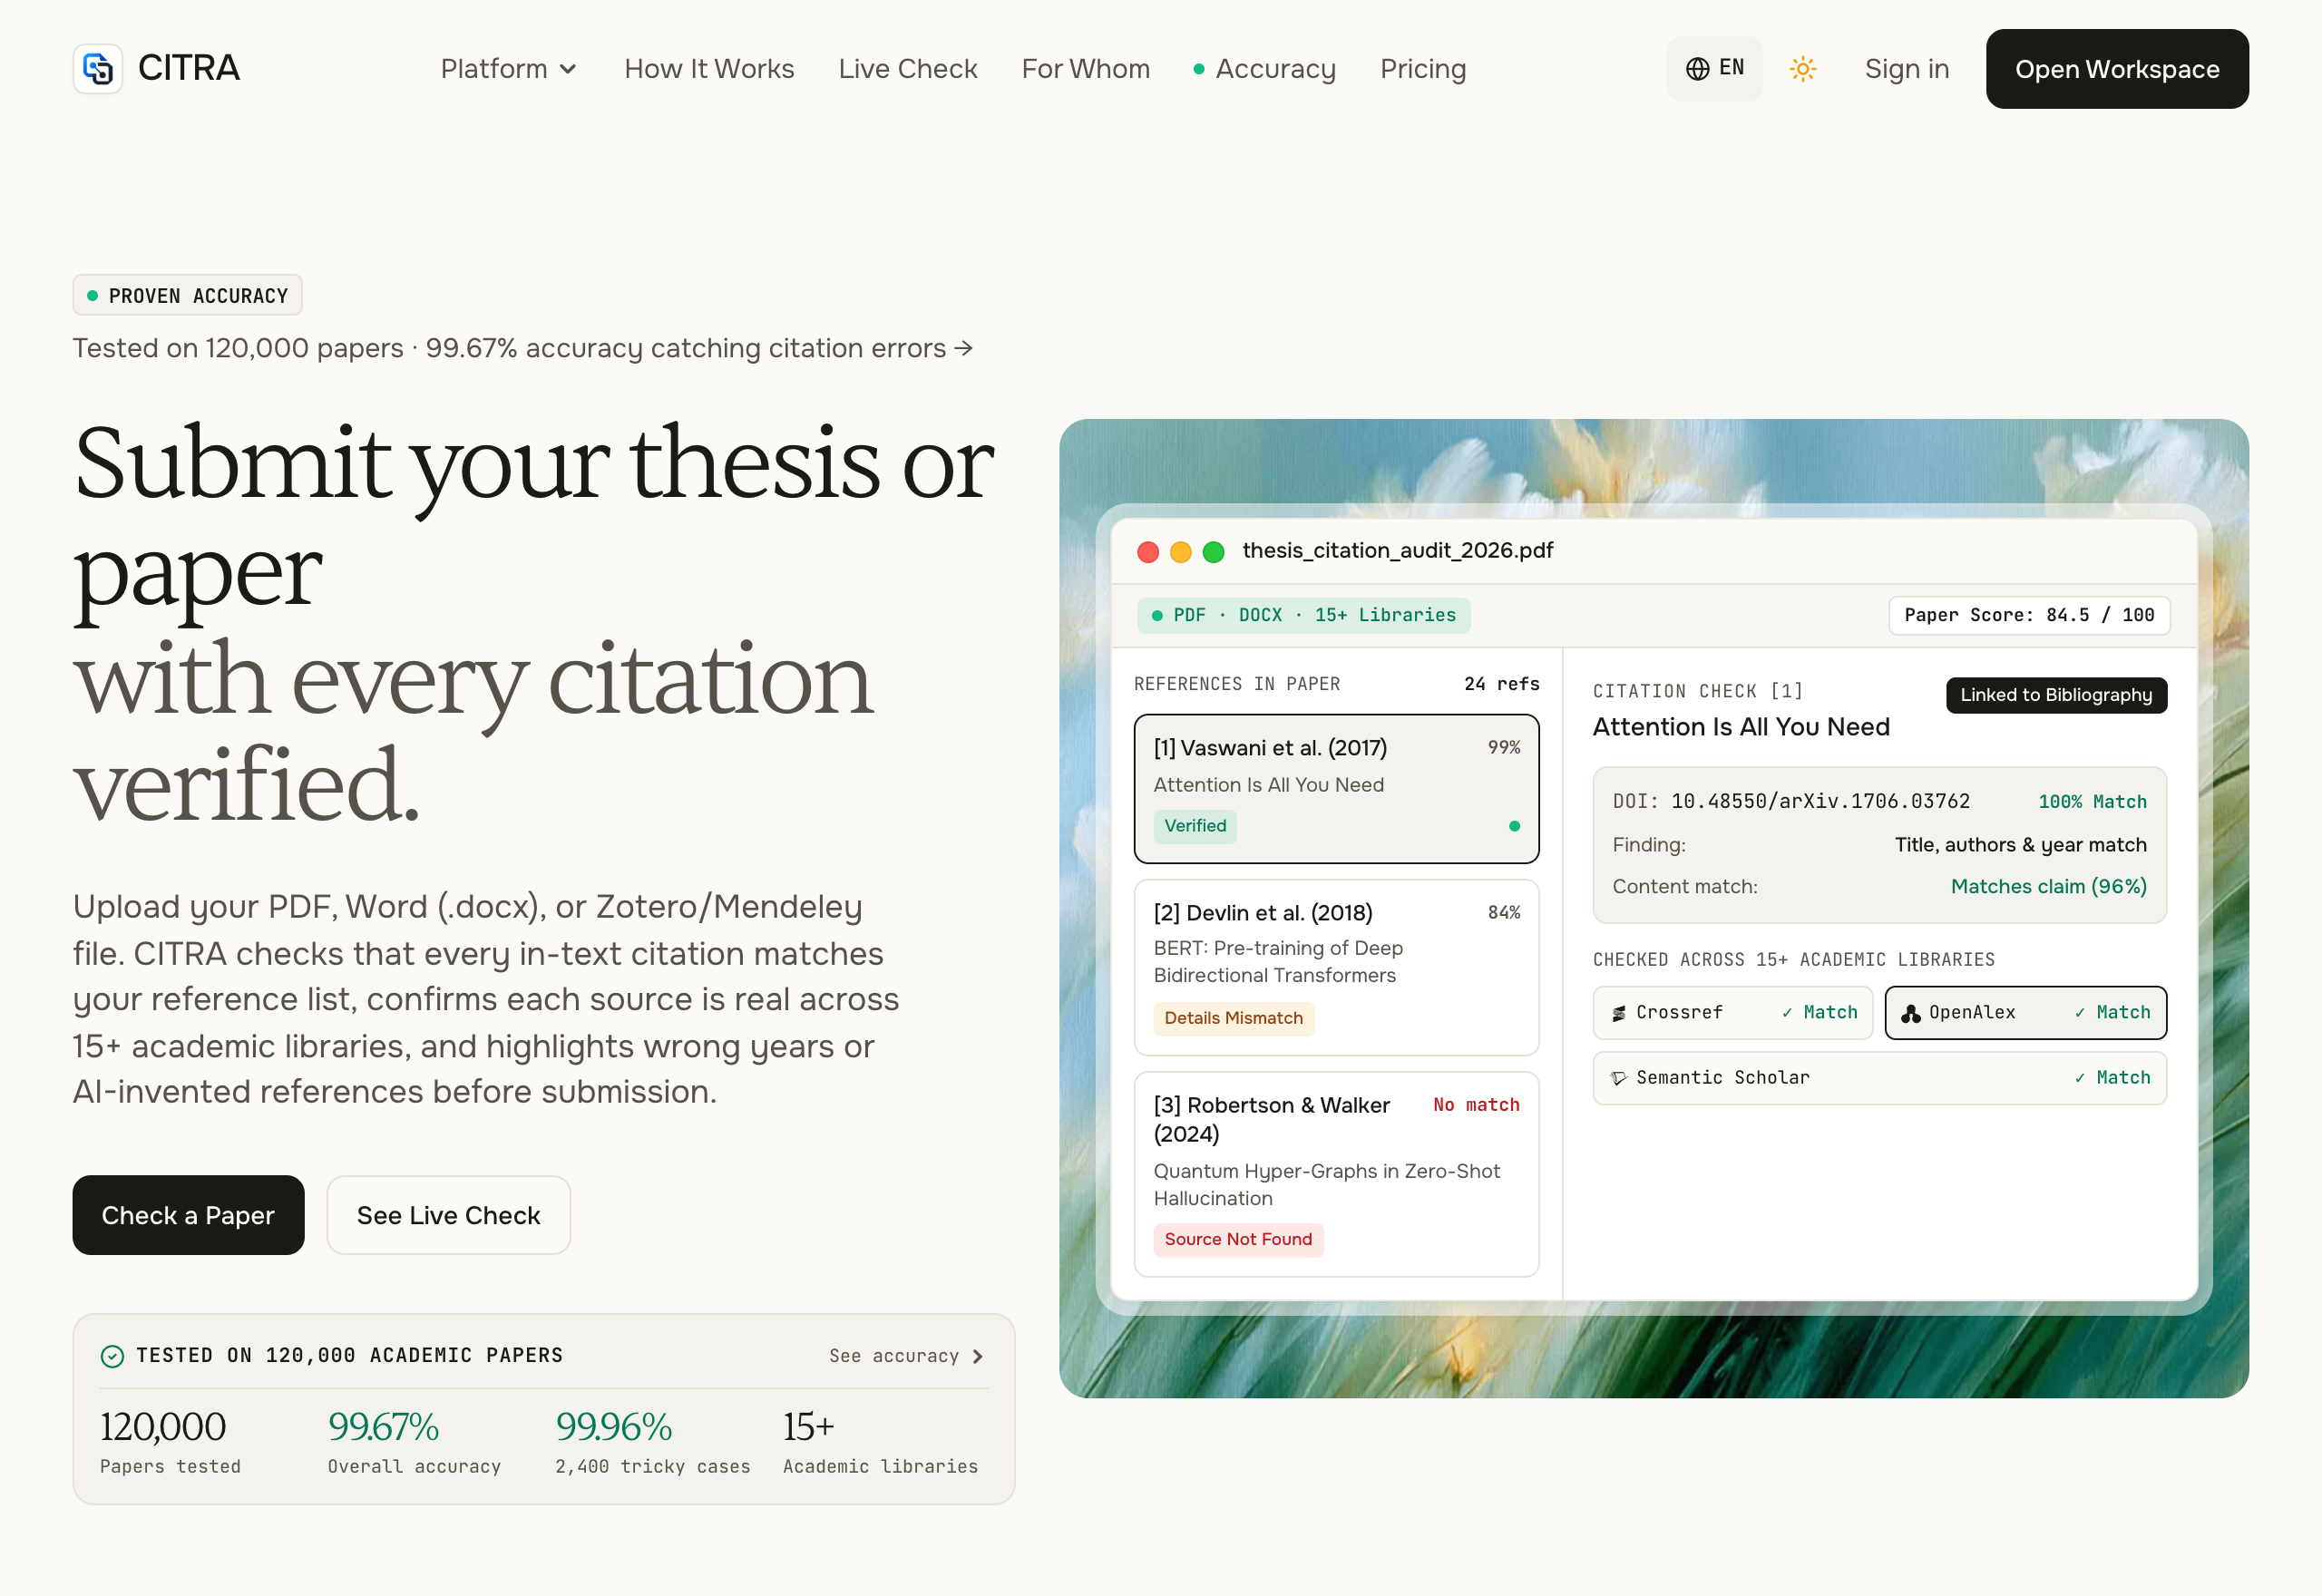
\includegraphics[width=0.49\textwidth,keepaspectratio]{picture/figures/01-landing-light.png}\hfill
    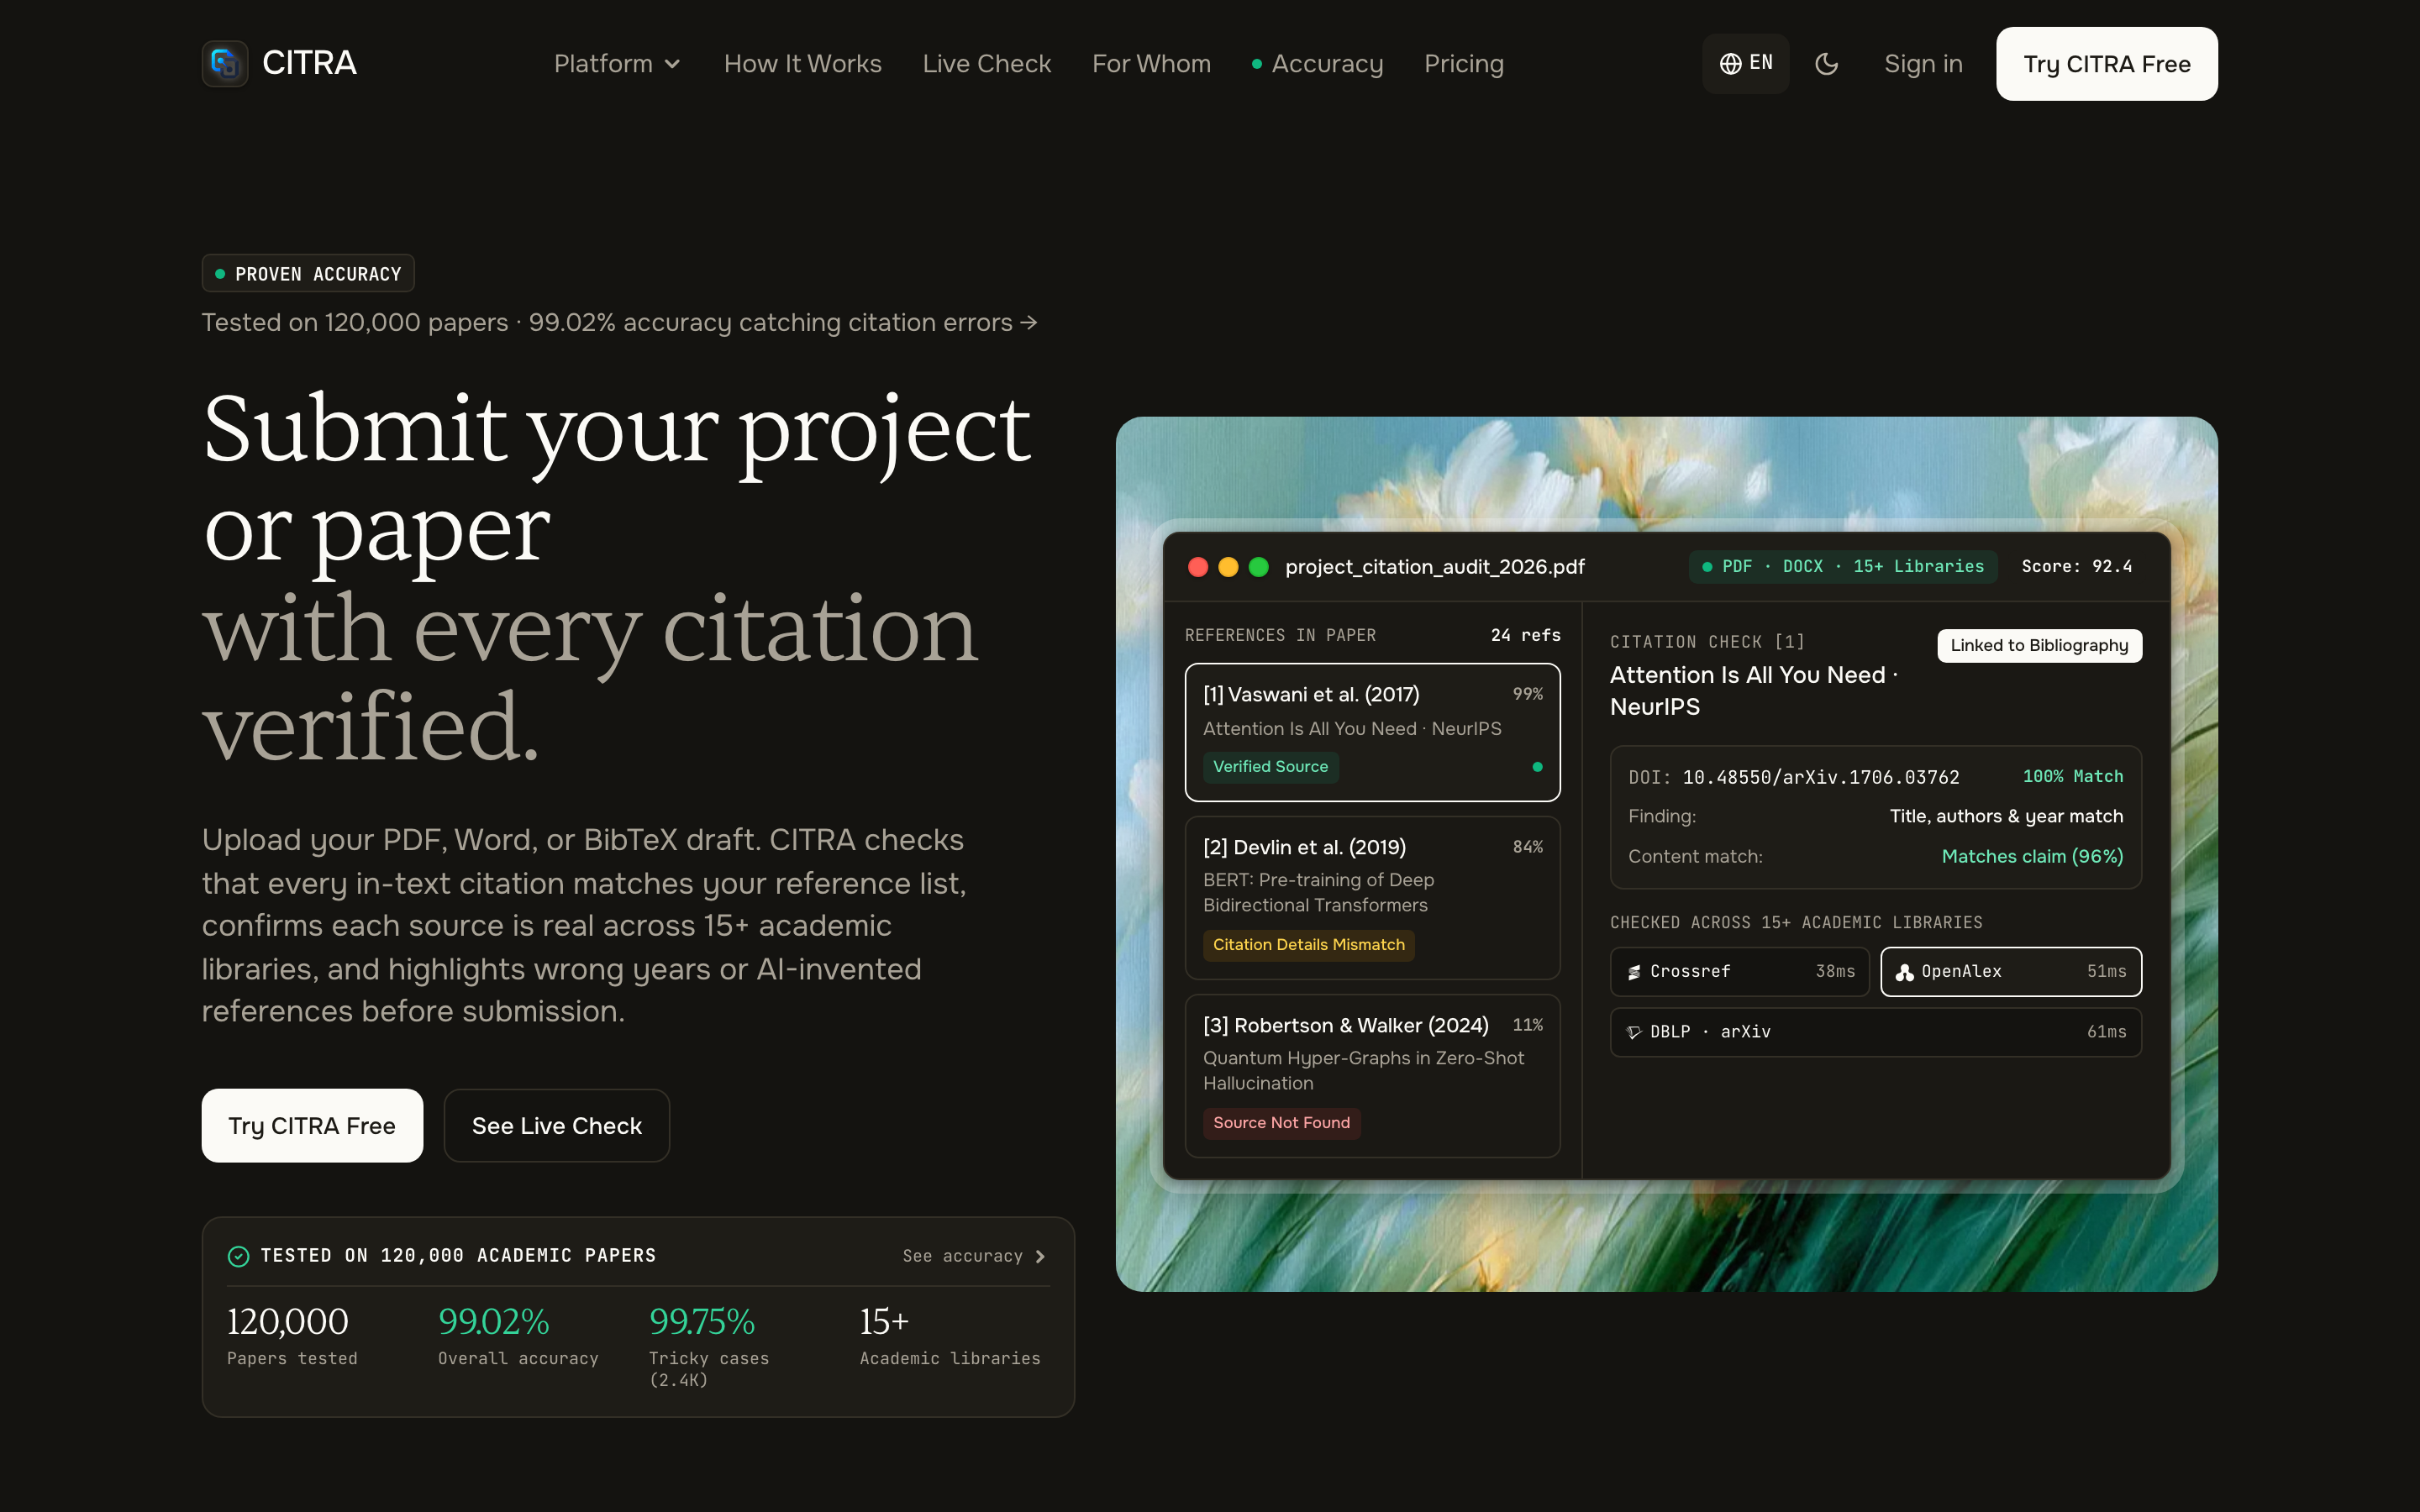
\includegraphics[width=0.49\textwidth,keepaspectratio]{picture/figures/02-landing-dark.png}
    \caption[CITRA landing page in WCAG AA Light and Dark themes]{CITRA (\texttt{v3.90.9}) public landing page rendered in Light mode (left) and Dark mode (right).}
    \label{fig:ui-landing}
\end{figure}

\begin{figure}[H]
    \centering
    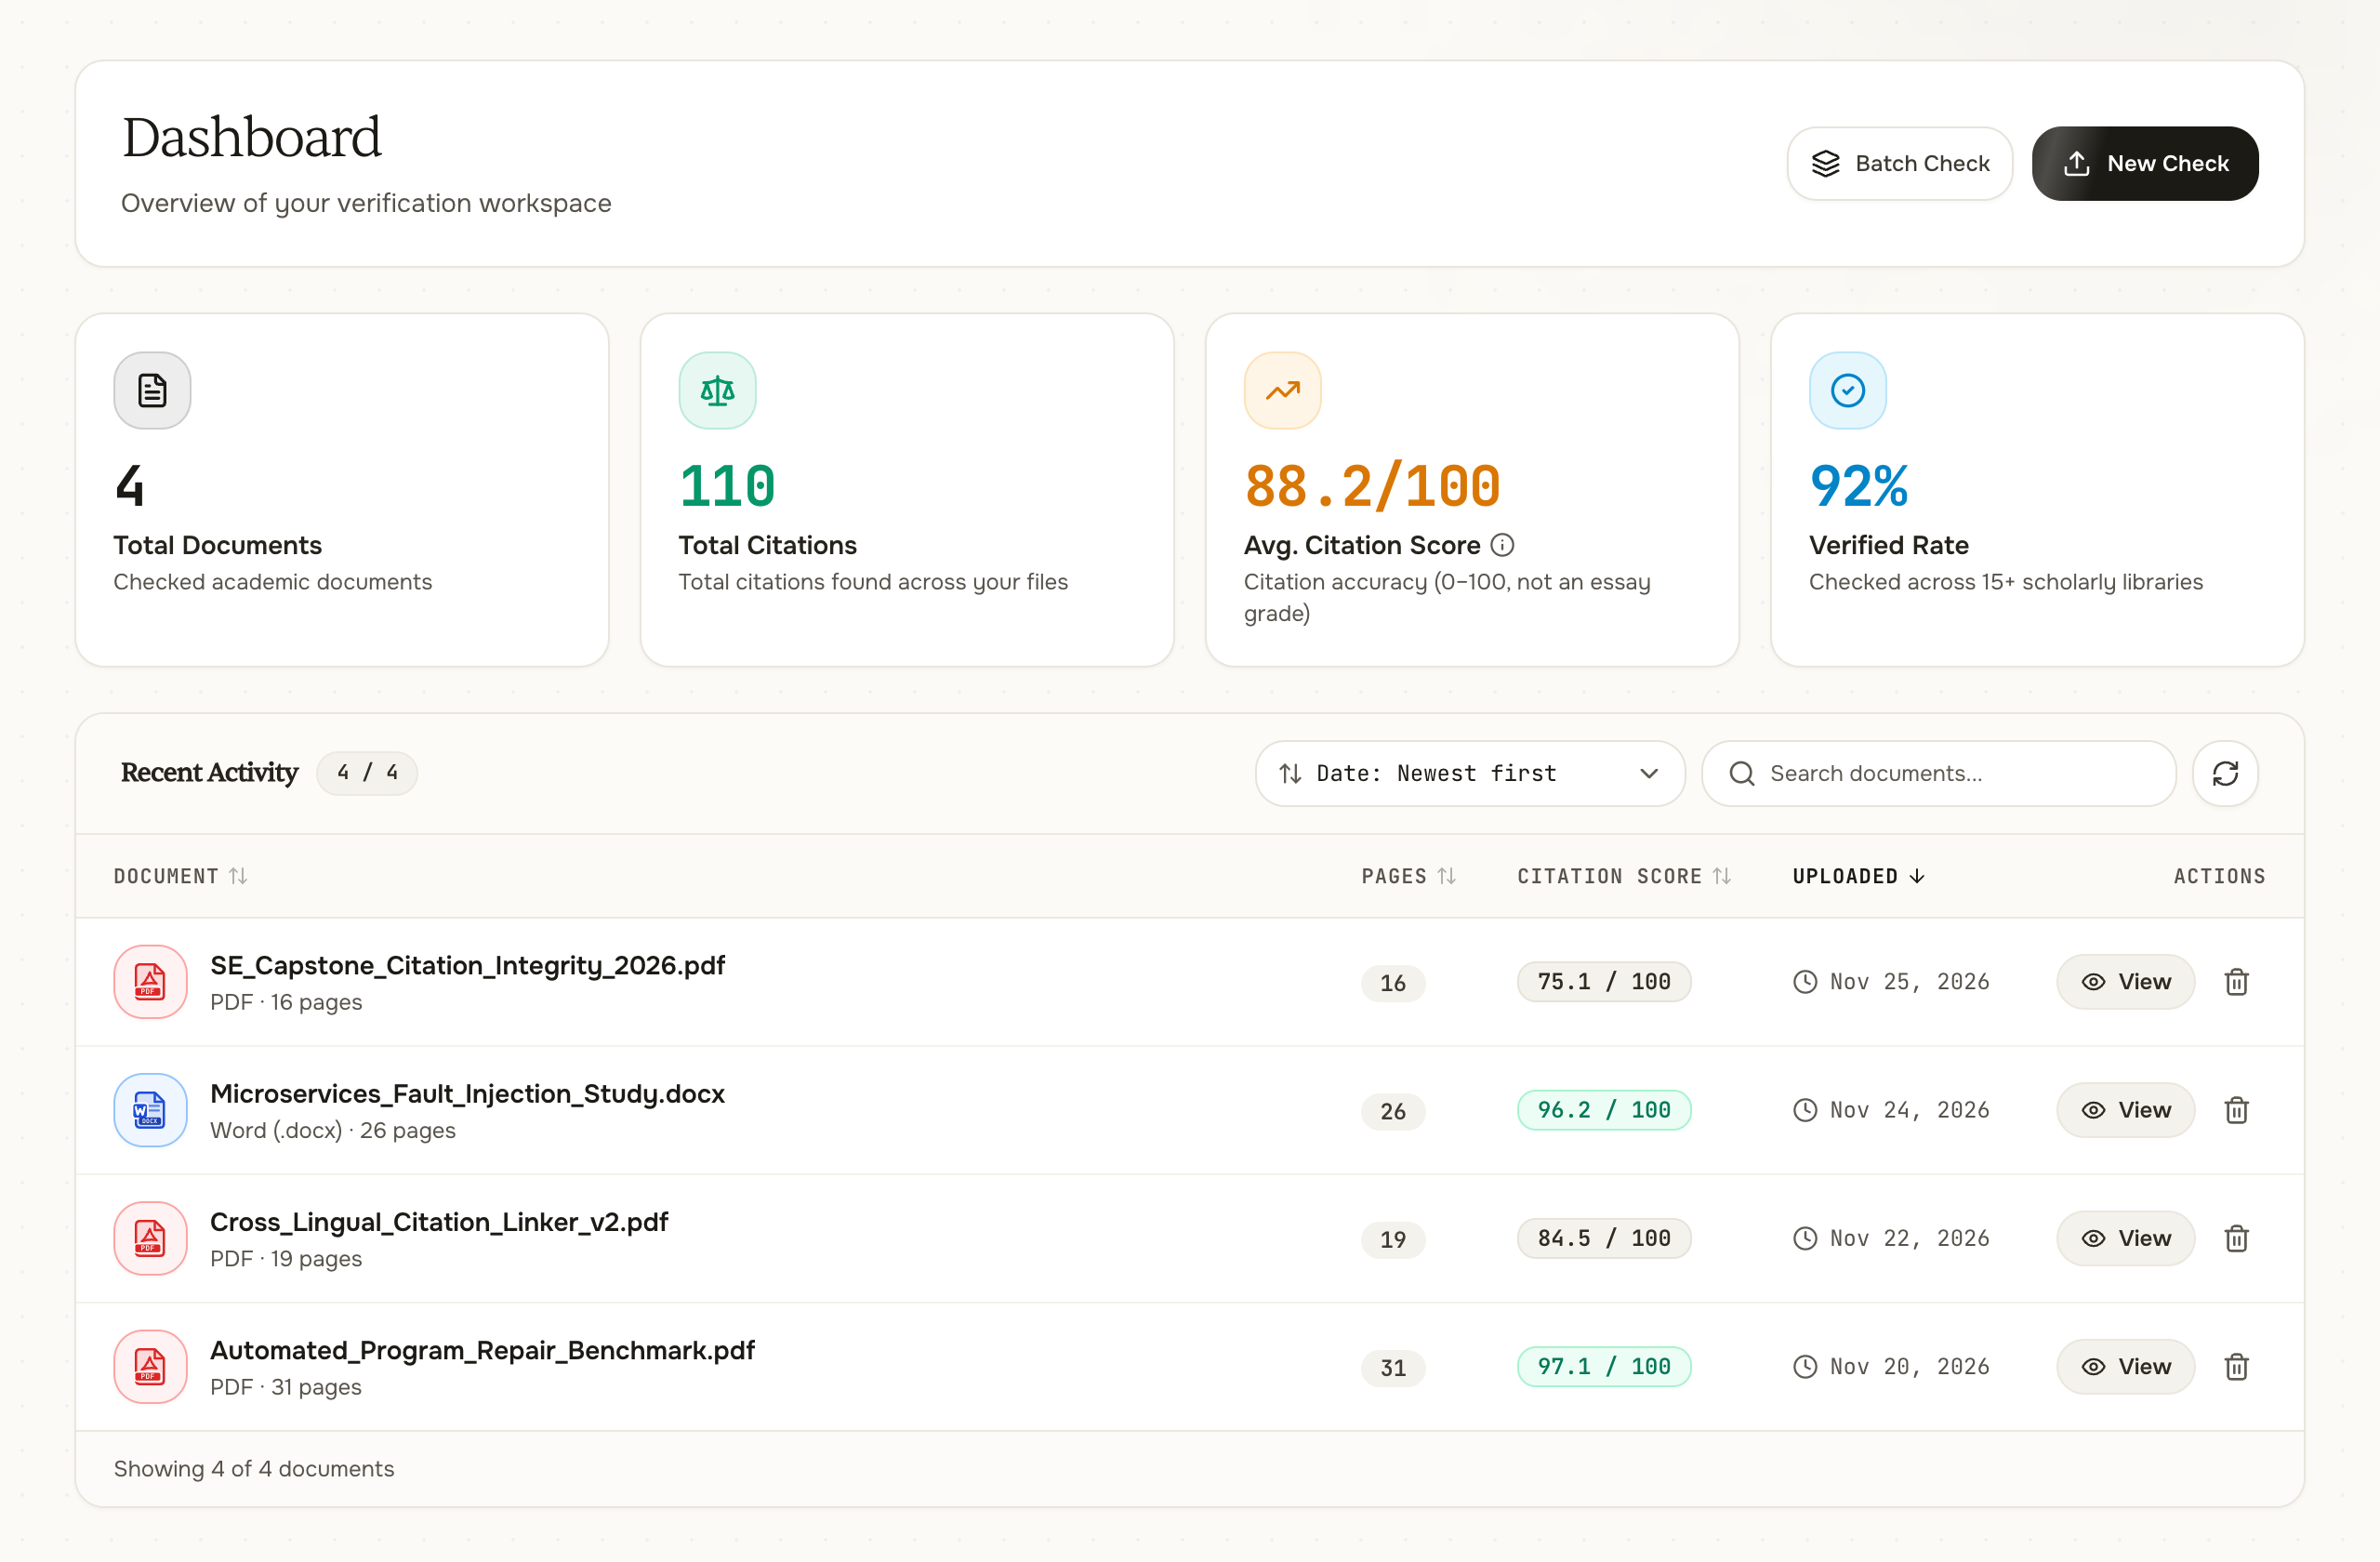
\includegraphics[width=0.49\textwidth,keepaspectratio]{picture/figures/03-dashboard-light.png}\hfill
    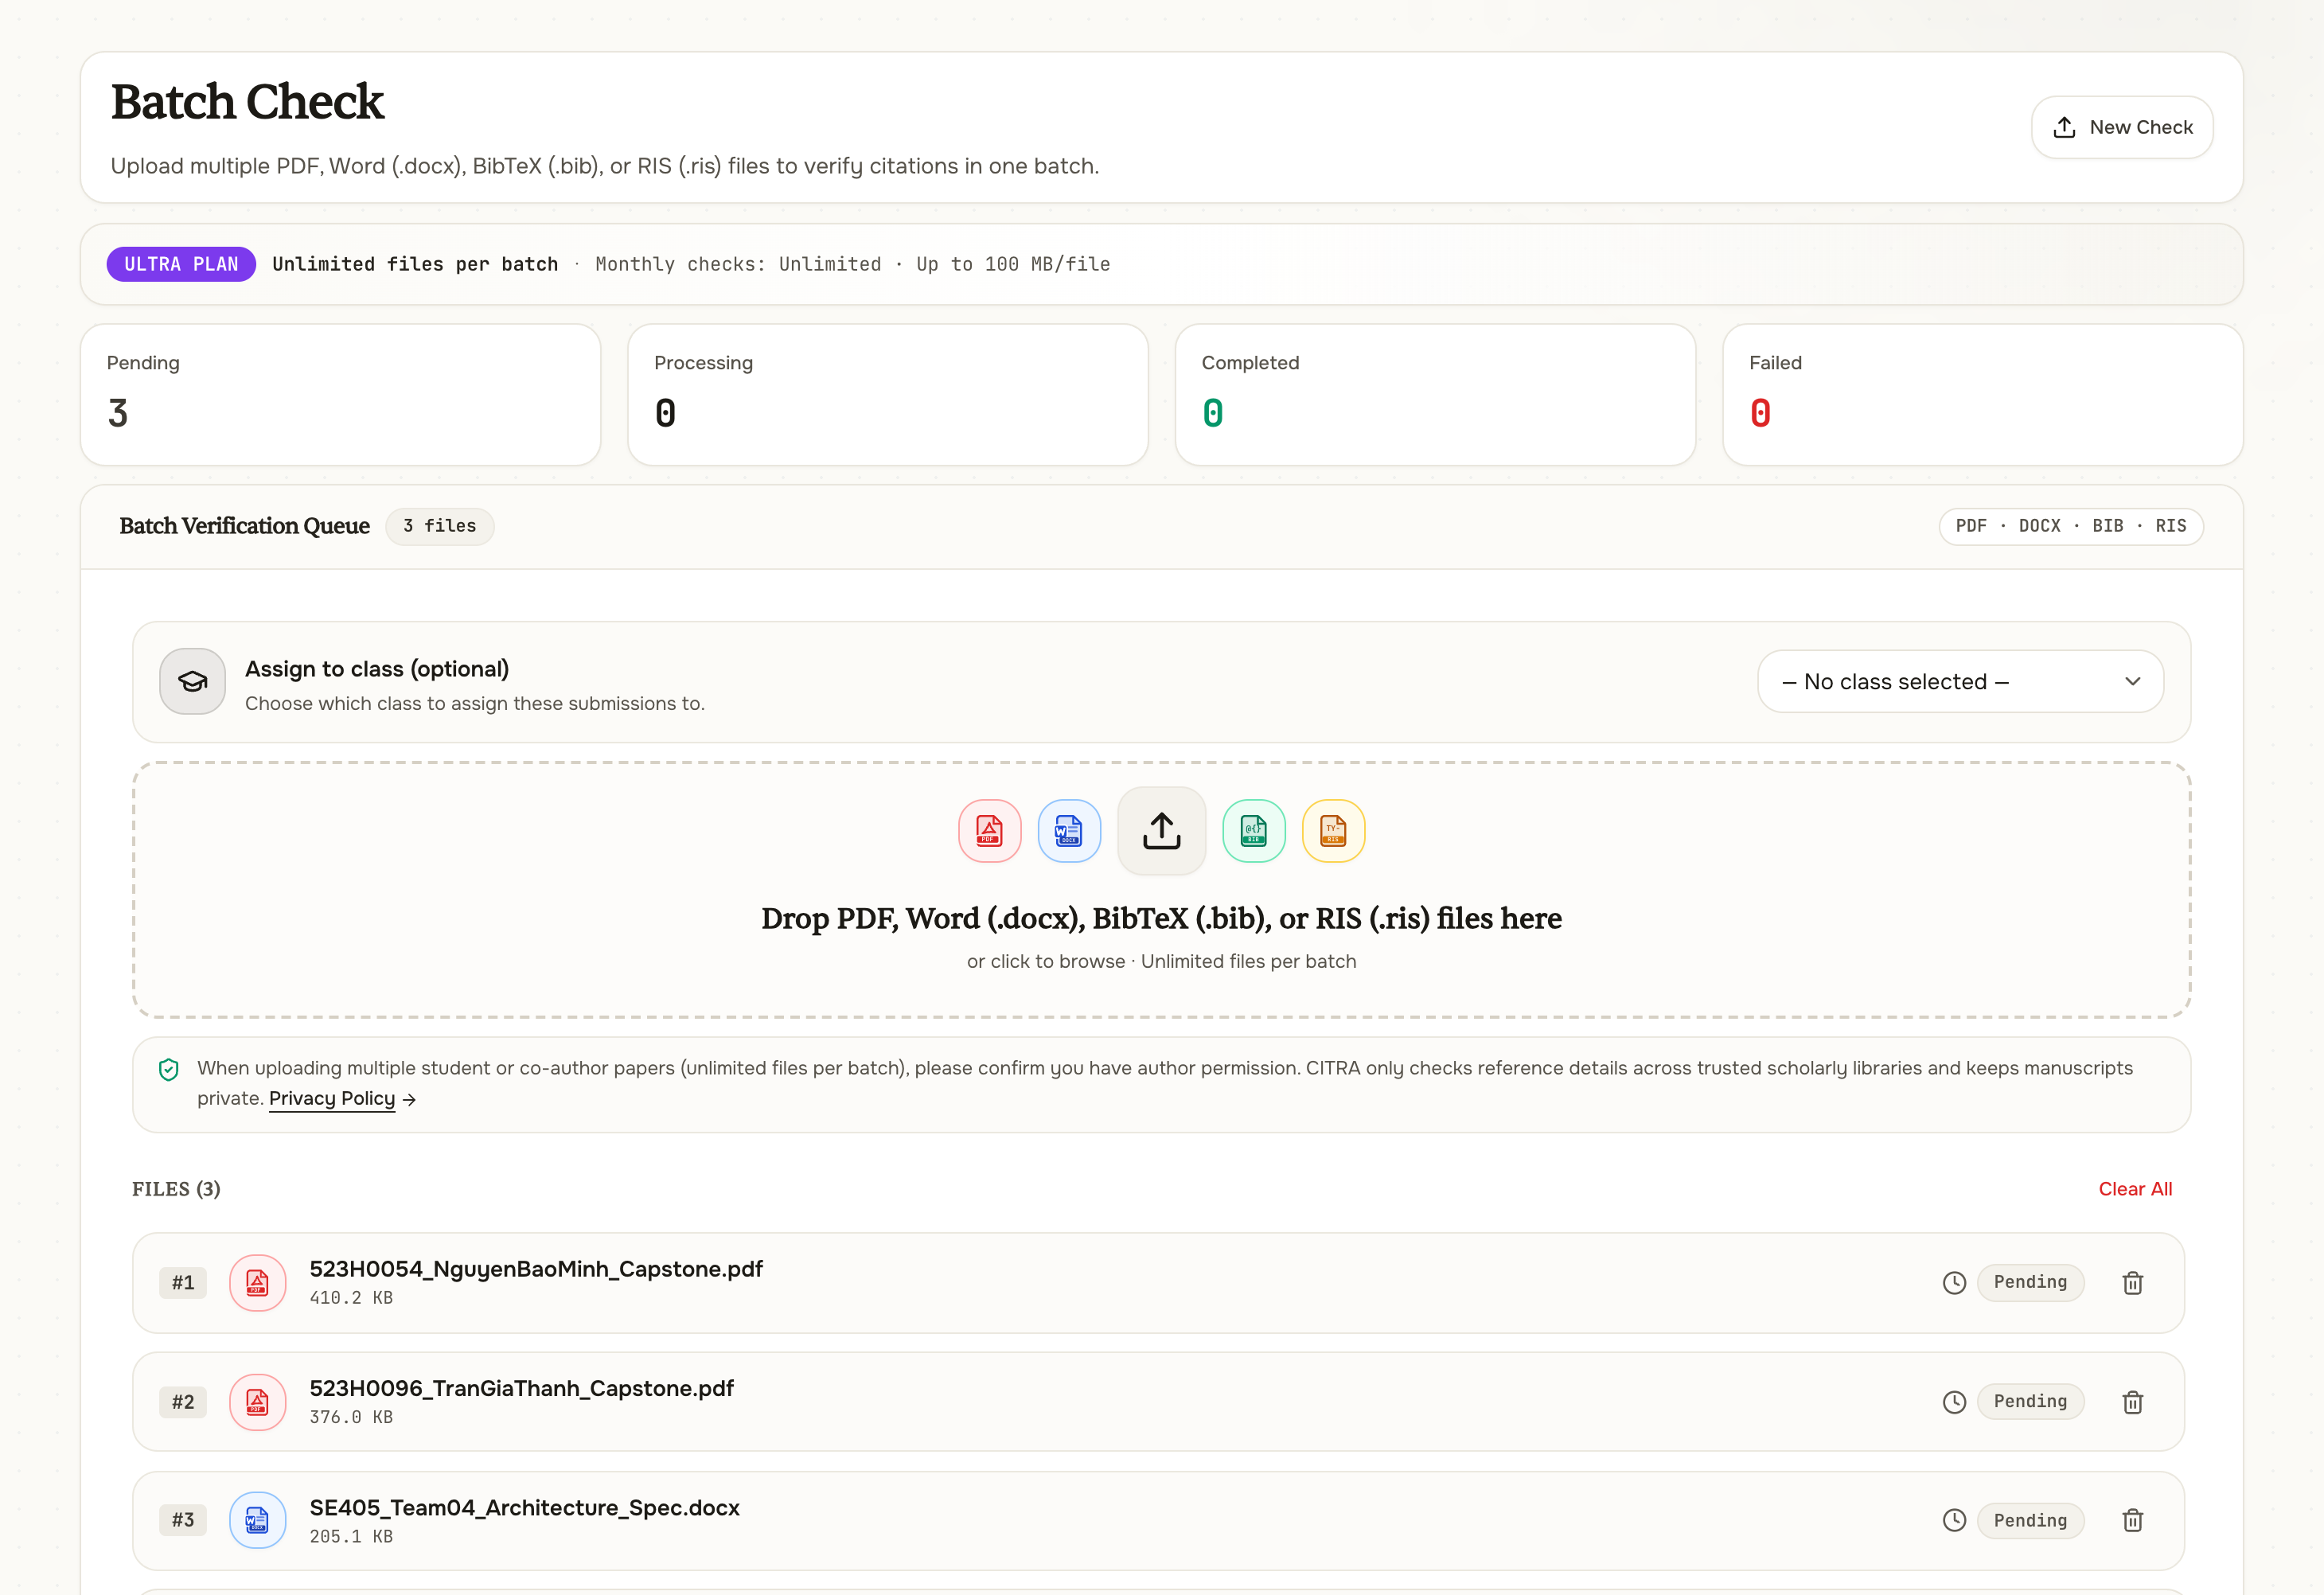
\includegraphics[width=0.49\textwidth,keepaspectratio]{picture/figures/04-batch-upload.png}
    \caption[Student verification dashboard and concurrent batch upload workspace]{Student verification dashboard (\texttt{/dashboard}, left) and multi-format batch verification queue (\texttt{/batch-upload}, right).}
    \label{fig:ui-workspace}
\end{figure}

\begin{figure}[H]
    \centering
    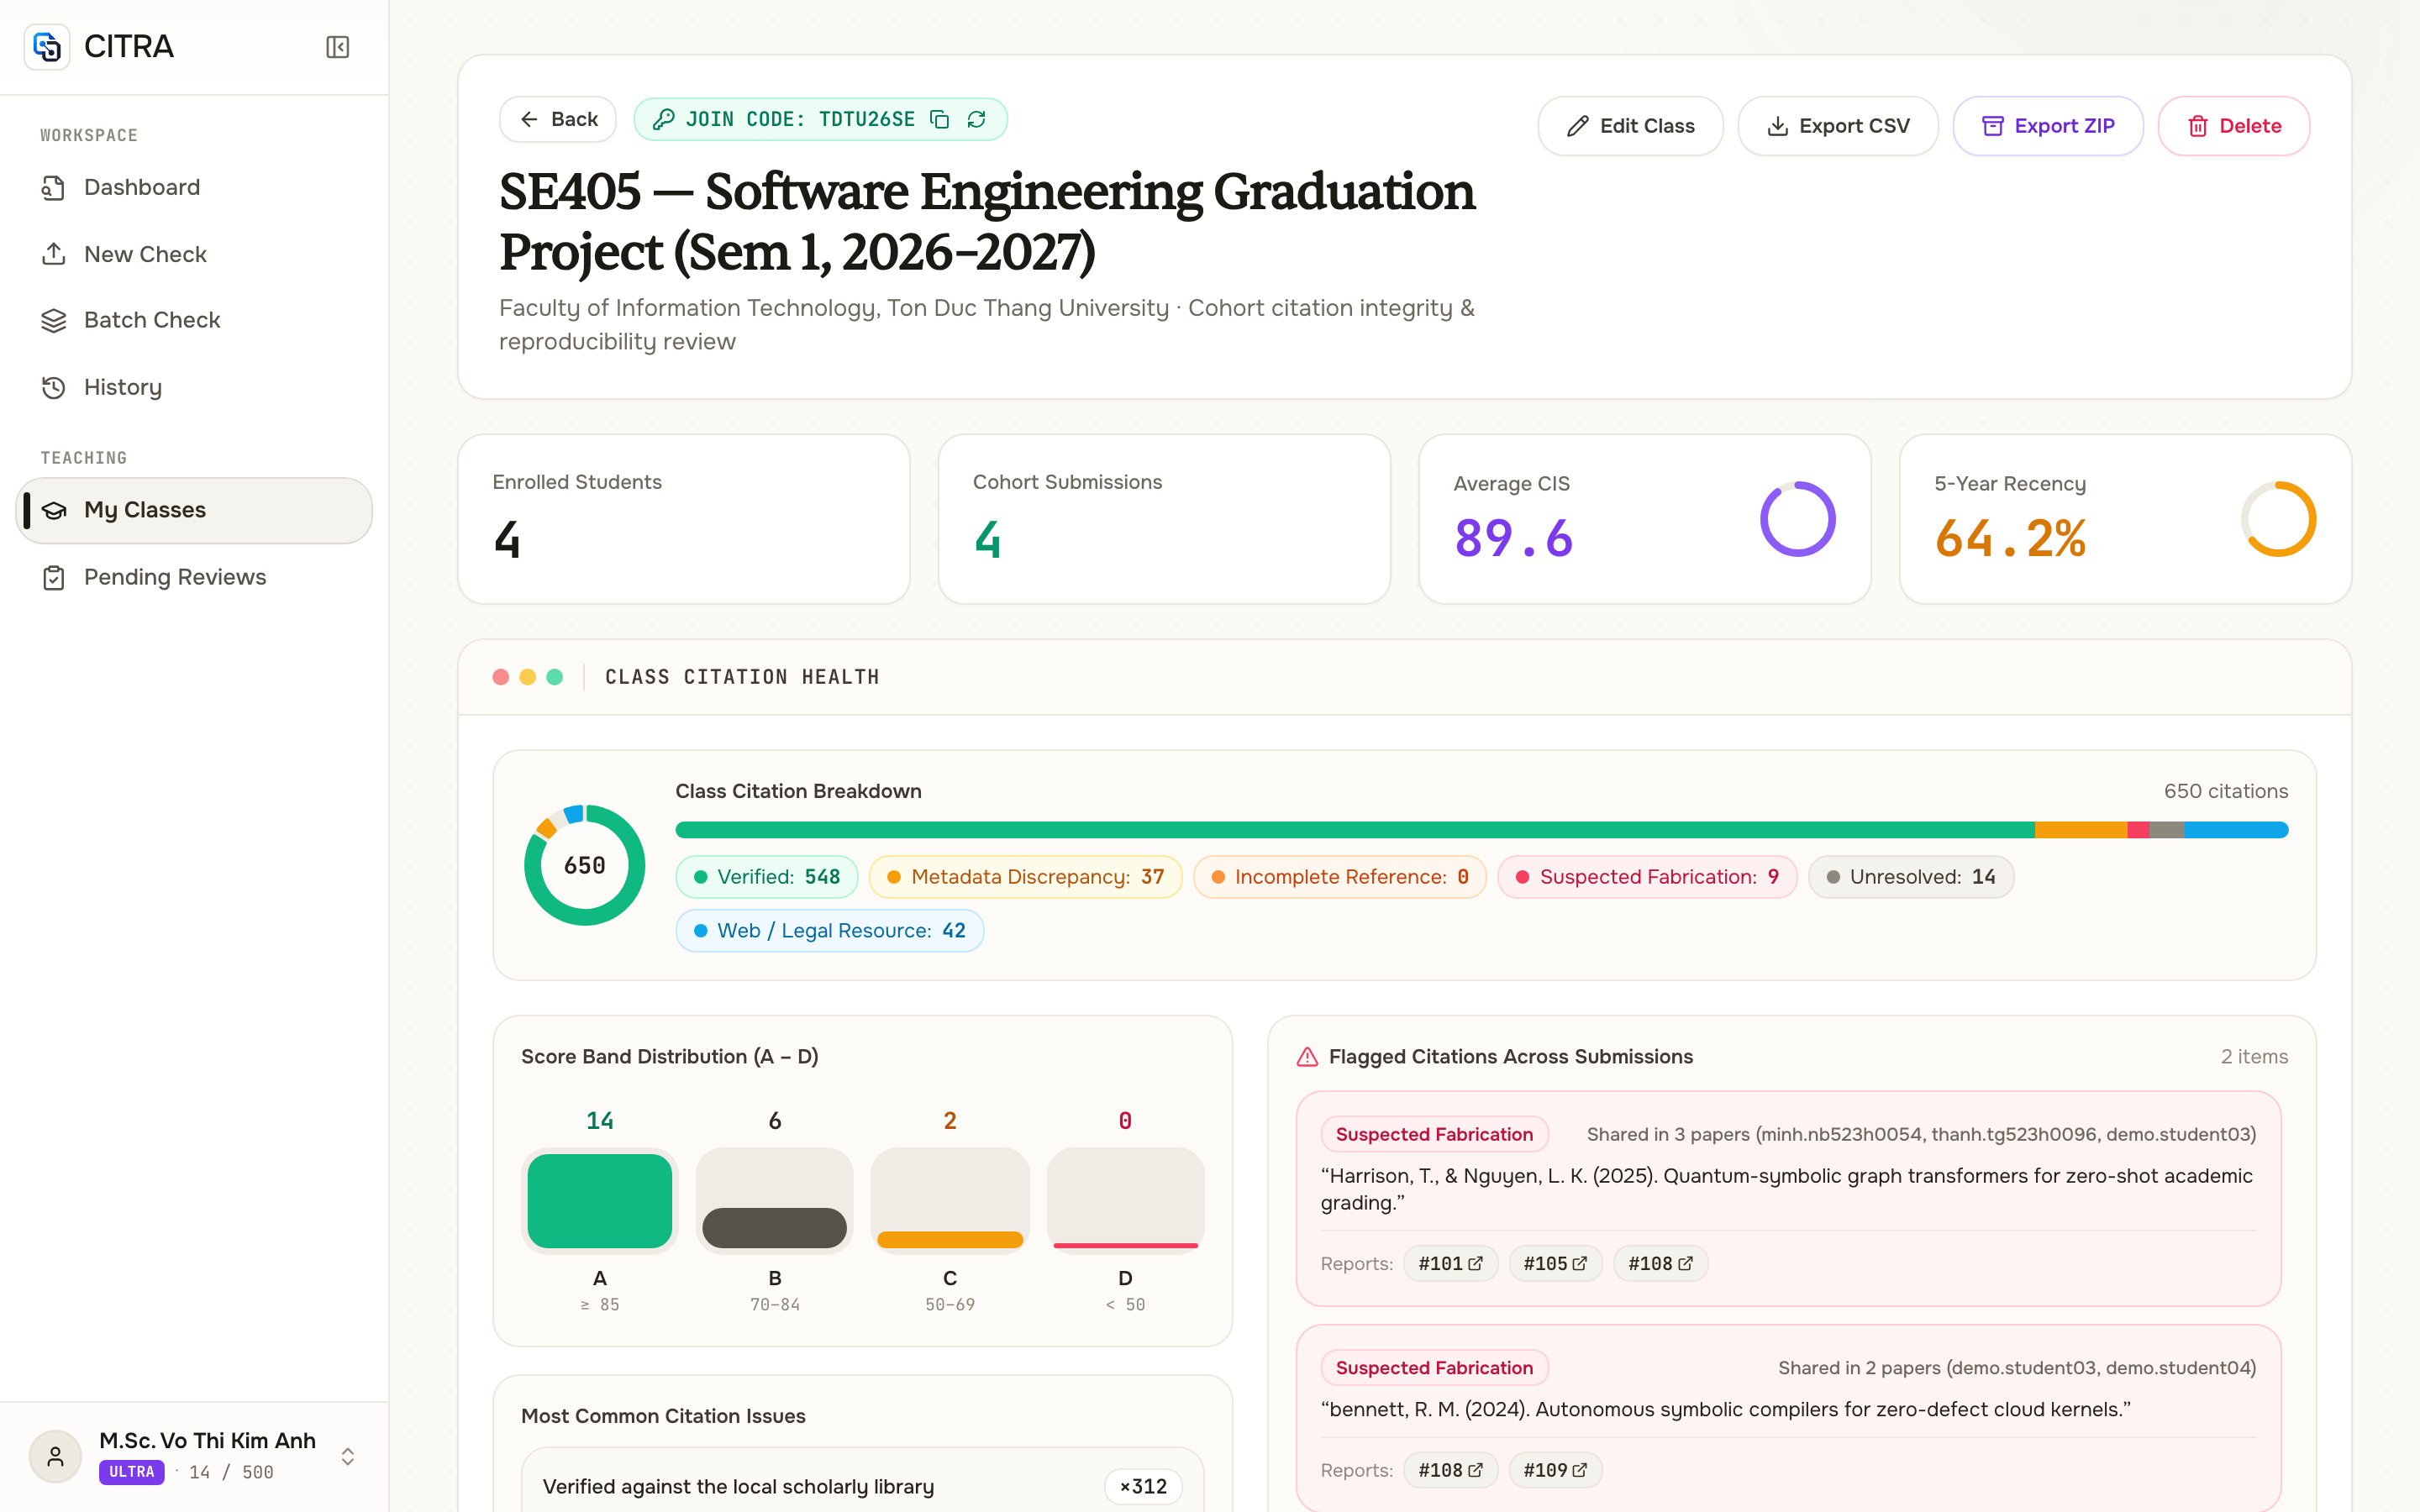
\includegraphics[width=0.49\textwidth,keepaspectratio]{picture/figures/10-teacher-classroom.png}\hfill
    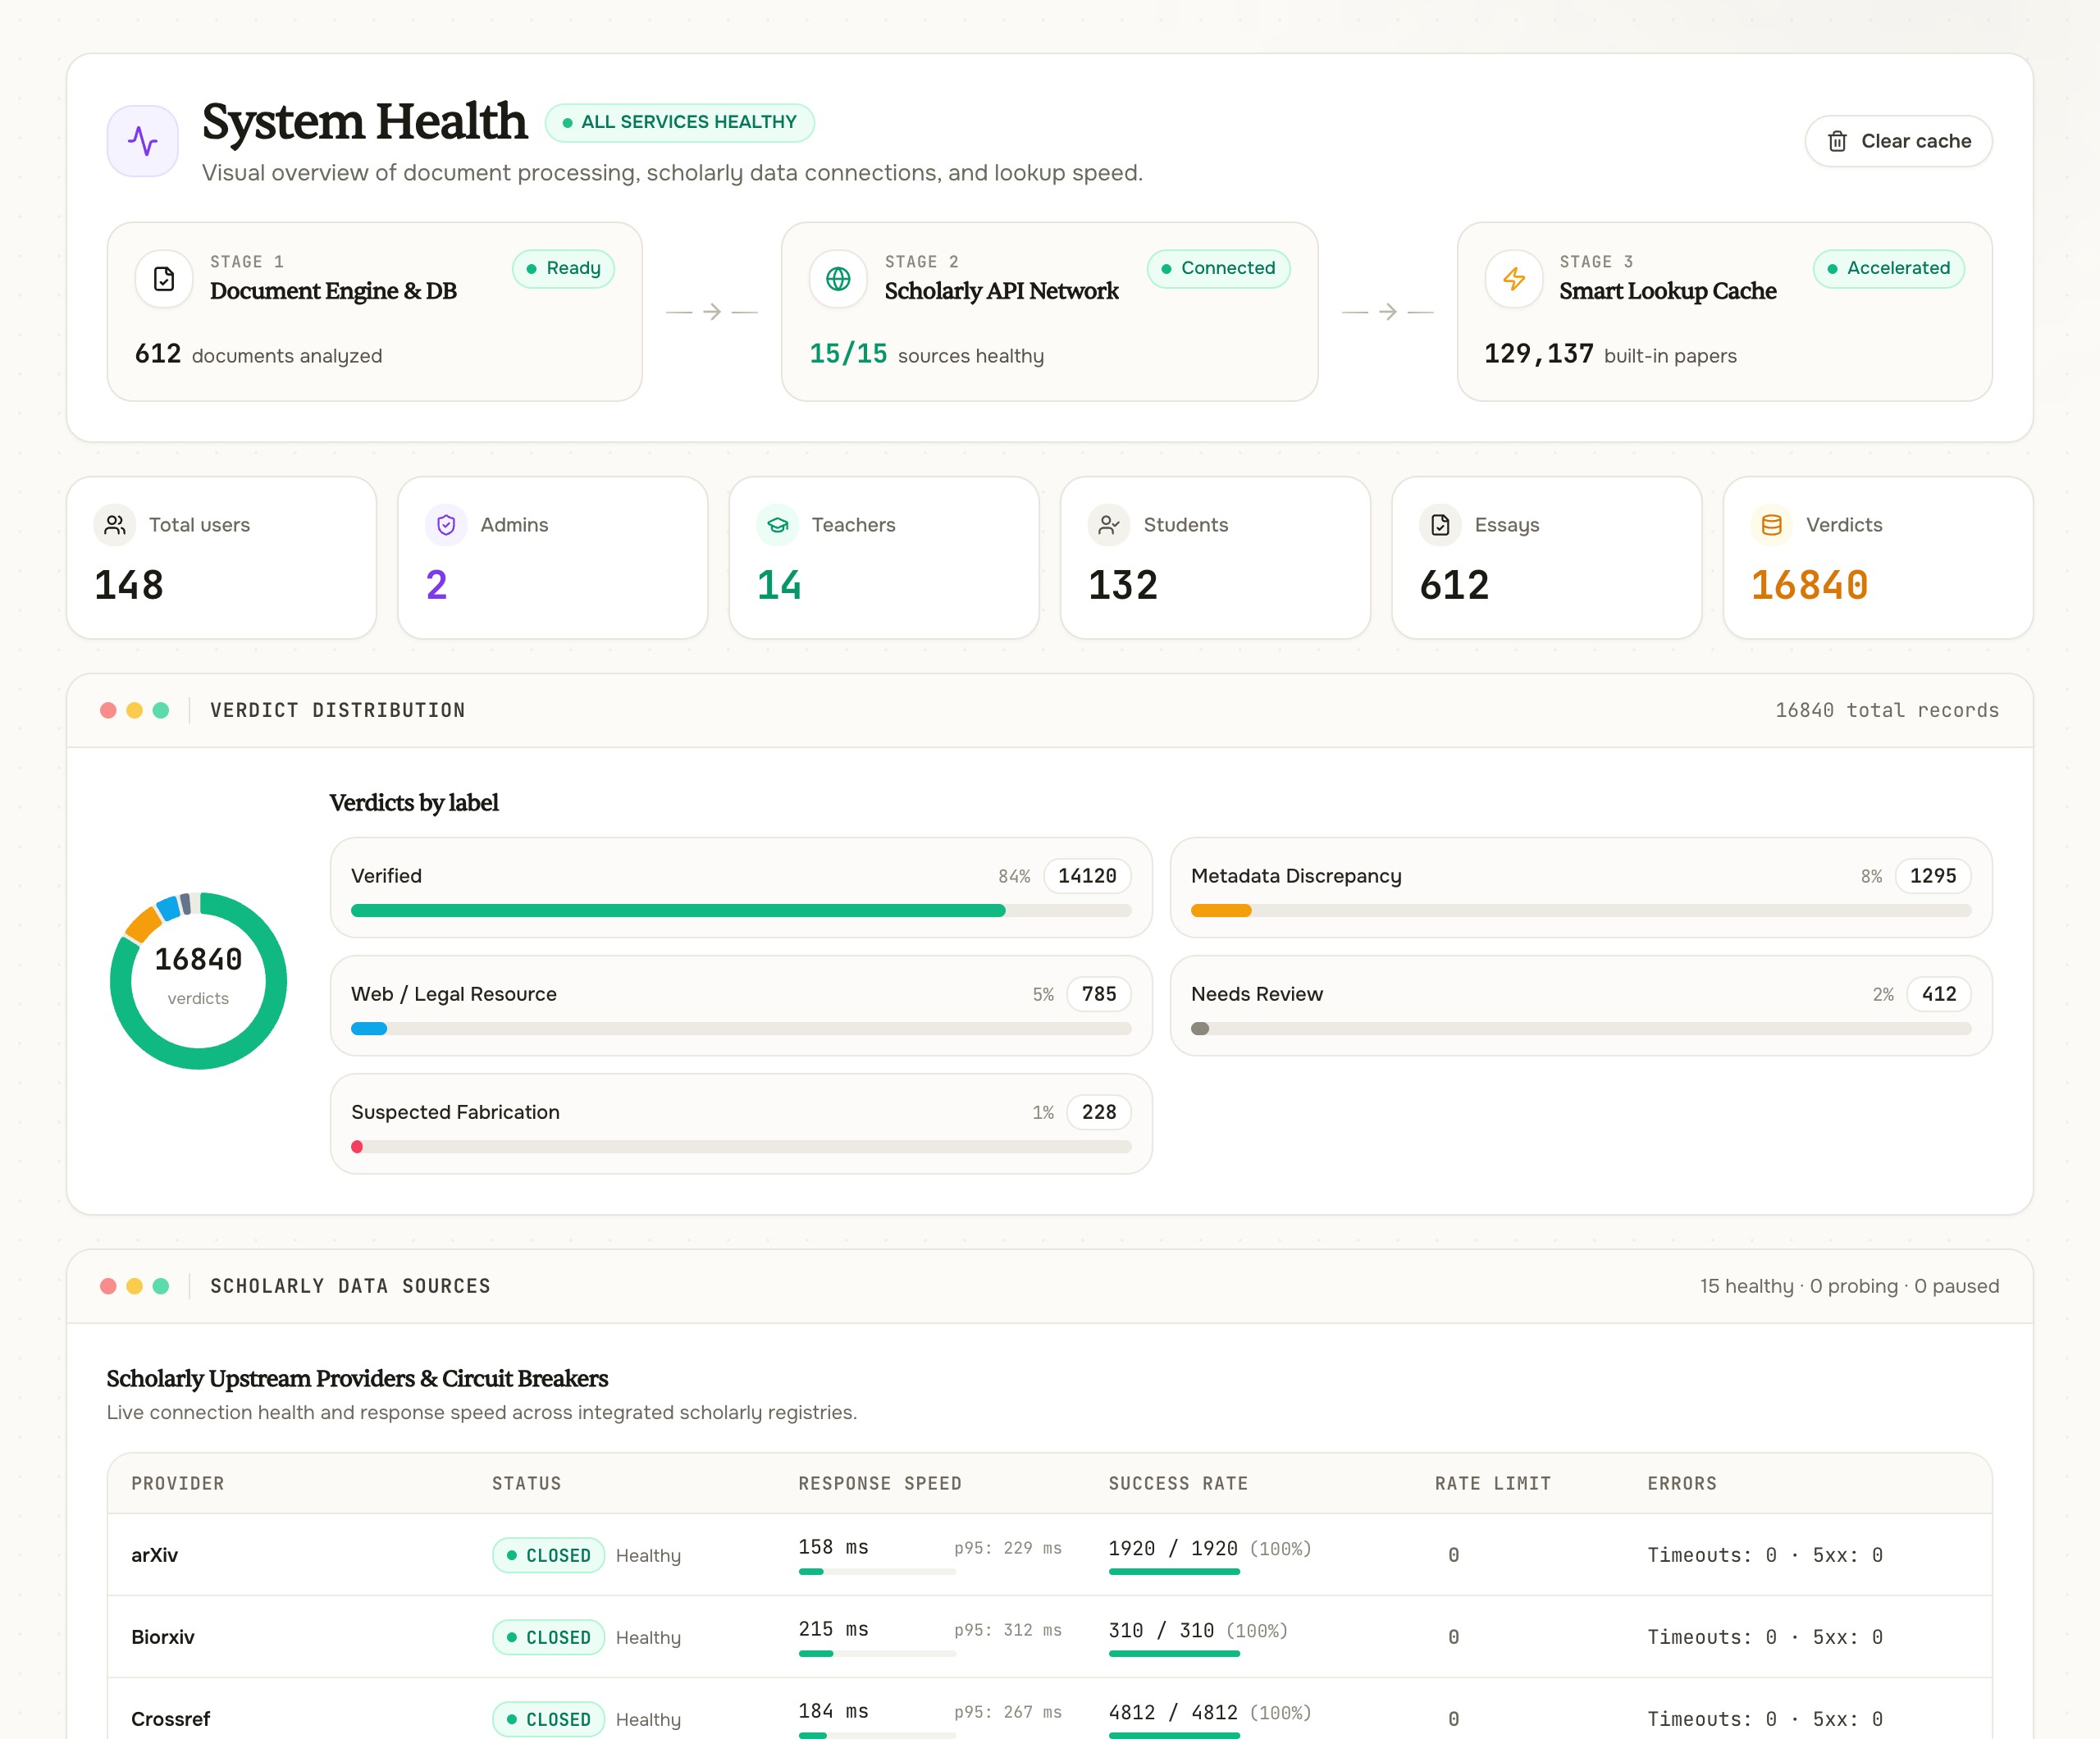
\includegraphics[width=0.49\textwidth,keepaspectratio]{picture/figures/11-admin-system-health.png}
    \caption[Teacher cohort analytics classroom and Administrator system health console]{Teacher classroom cohort analytics (\texttt{/teacher/classes/1}, left) and Administrator system health monitor (\texttt{/admin/system}, right).}
    \label{fig:ui-portals}
\end{figure}

\section{Chapter Summary}

This chapter presented the implementation of \textbf{CITRA} across its eight software layers: multi-format 12-style extraction, work-level merging and 7-method bidirectional linking, tiered 15-API retrieval with pinned-IP URL/HTML validation, dual-encoder \texttt{VI}$\leftrightarrow$\texttt{EN} semantic matching, 68-rule neuro-symbolic verification with 16D Logistic Regression and Platt scaling, five-component CIS grading, and the code-split React workspace. Chapter~\ref{chap:results} evaluates these components empirically across five research questions.
